% Editorial v52. Recorded v47 evaluation and v52 post-hoc controls.
\PassOptionsToPackage{table}{xcolor}
\documentclass{article}

\usepackage{iclr2027_conference,times}
\input{math_commands.tex}

\usepackage{hyperref}
\usepackage{xurl}
\usepackage{graphicx}
\usepackage{epstopdf}
\epstopdfsetup{outdir=build/}
\usepackage{booktabs}
\usepackage{amsmath}
\usepackage{amssymb}
\usepackage{multirow}
\usepackage{array}
\usepackage{tabularx,adjustbox}
\usepackage{xcolor}

\definecolor{phgray}{gray}{0.45}
\definecolor{bestgray}{gray}{0.94}

\newcommand{\best}[1]{\textbf{#1}}
\newcommand{\second}[1]{\underline{#1}}
\newcommand{\oracle}[1]{\textit{\textcolor{phgray}{#1}}}
\newcommand{\introact}{\textsc{IntroAct-TS}}
\newcommand{\tsfm}{TSFM}
\newcommand{\calA}{\mathcal{A}}
\newcommand{\calB}{\mathcal{B}}
\newcommand{\calN}{\mathcal{N}}
\newcommand{\loss}{\ell}

\newcommand{\fix}{\marginpar{FIX}}
\newcommand{\new}{\marginpar{NEW}}

\setlength{\parskip}{3.8pt plus 1pt minus 0.5pt}

\setlength{\textfloatsep}{5pt plus 2pt minus 2pt}
\setlength{\floatsep}{5pt plus 2pt minus 2pt}
\setlength{\intextsep}{5pt plus 2pt minus 2pt}
\setlength{\abovedisplayskip}{5pt plus 2pt minus 2pt}
\setlength{\belowdisplayskip}{5pt plus 2pt minus 2pt}
\setlength{\abovedisplayshortskip}{3pt plus 1pt minus 1pt}
\setlength{\belowdisplayshortskip}{3pt plus 1pt minus 1pt}
\setcounter{topnumber}{4}
\setcounter{bottomnumber}{3}
\setcounter{totalnumber}{5}
\renewcommand{\topfraction}{0.92}
\renewcommand{\bottomfraction}{0.65}
\renewcommand{\textfraction}{0.06}
\renewcommand{\floatpagefraction}{0.72}

\title{\introact{}: Selective Input Governance for \\
Frozen Time-Series Foundation Models}

\author{Anonymous Authors\\Paper under double-blind review}

\begin{document}

\maketitle

\begin{abstract}
A deployed time-series foundation model may receive contexts with missing observations.
Whether a repair improves its forecast varies from request to request, so the system must
choose among candidate repairs and the unchanged input. We introduce \introact{}, which makes
this choice for each request while preserving observed values and model parameters. It
executes a fixed catalog of repairs on historical windows and records their forecasting
utilities relative to the unchanged input. At deployment, it estimates each action's utility
from similar historical states and intervenes only when a dispersion-penalised score is
positive; otherwise, it returns the reference forecast. An evaluation using previously
examined test data covers eight sources, three frozen backbones, four missingness patterns
and two horizons. At $10\%$ missingness, source-macro MASE is 1.437 against 1.576 for the
unchanged input, with paired intervals excluding zero on all three backbones, and harmful
loss is 0.0375 against 0.0513 for the best fixed repair. The margin over the stronger simple
controls is concentrated in one source, a per-source fixed policy is at least as accurate on
two of the three backbones, and frequency-matched controls expose an accuracy--harm tradeoff
rather than uniformly lower harm. Because earlier results on this test data informed the
design, these findings are exploratory and require independent confirmation.

\end{abstract}

\section{Introduction}
\label{sec:intro}

Time-series foundation models (\tsfm{}s) support forecasting without task-specific
retraining~\citep{ansari2024chronos,chronosbolt2025,das2024timesfm,woo2024moirai,chronos2_2025},
but the context they receive at deployment may contain missing observations caused by sensor
outages or delayed measurements~\citep{chen2024bitgraph,peng2025s4m}. We study input
processing for a fixed predictor under one constraint: every valid observation is preserved.
Within this constraint, a repair can fill the unobserved positions, and whether to use the
repaired input must be judged by its effect on the forecast. The question is which repair an
incomplete request should receive, and when the input should be left unchanged.

Missing inputs have been handled at different stages. Imputation methods reconstruct missing
values from temporal or cross-channel
structure~\citep{cao2018brits,tashiro2021csdi,du2023saits}, and missingness-aware forecasters
learn to use incomplete contexts during training~\citep{chen2024bitgraph,peng2025s4m}.
Rather than scoring reconstruction, task-oriented imputation evaluates a repair by its
downstream effect~\citep{wang2024taskoriented,hao2025toivsf,xu2026srdi}, and for frozen
forecasters TATO selects transformation pipelines from historical task
performance~\citep{qiu2026tato}. We adopt downstream forecasting performance as the criterion
and study a finer decision: within a fixed catalog, different requests may receive different
repairs, or none.

The value of a repair is the change in forecasting loss relative to leaving the input
unchanged, and it varies with the request and the frozen backbone. A repair can recover a
local pattern yet increase forecasting loss, while the backbone's native handling of missing
values may already be adequate. At deployment the future target is unavailable, so this
utility cannot be measured when the decision is made. For historical windows the target has
already been observed, so every admissible action can be executed on the same window and
compared pairwise against the unchanged input. The resulting utility labels provide the
supervision that repair selection needs; what remains is to estimate, from these labels, what
each action will do for a new request.

\introact{} uses these historical utility labels to make a repair decision for each request.
Offline, it stores each action's realised utility together with the state used for retrieval.
Online, it retrieves nearby historical records for each action and computes a local mean
utility and its dispersion. It subtracts a dispersion penalty from the mean and executes the
highest-scoring repair only when its score is positive; otherwise it returns the cached
reference forecast. The procedure uses one forecasting-backbone call for the reference and at
most one additional call for the selected repair. Candidate inputs are constructed before
selection, and their costs are accounted for separately. Figure~\ref{fig:concept} illustrates
the procedure.

The paper makes three contributions. First, it formulates missing-input handling for a frozen
forecaster as per-request action selection, with the unchanged input inside the decision
space. Second, it supports this choice with historical full-action replay: utility labels
relative to \textsc{Keep}, an action-specific local estimator, and a dispersion-penalised
decision rule. Third, it evaluates the rule across eight sources and three frozen backbones
against fixed repairs and simple selection strategies, reporting forecast error, intervention
harm and computational cost, and retaining the unfavourable comparisons.

One property of the evaluation bounds these findings: earlier results on the same test data
informed the current design. The reported comparisons are therefore exploratory rather than
independent confirmation, and \S\ref{sec:exp-setup} states the boundary precisely.

\begin{figure}[t]
  \centering
  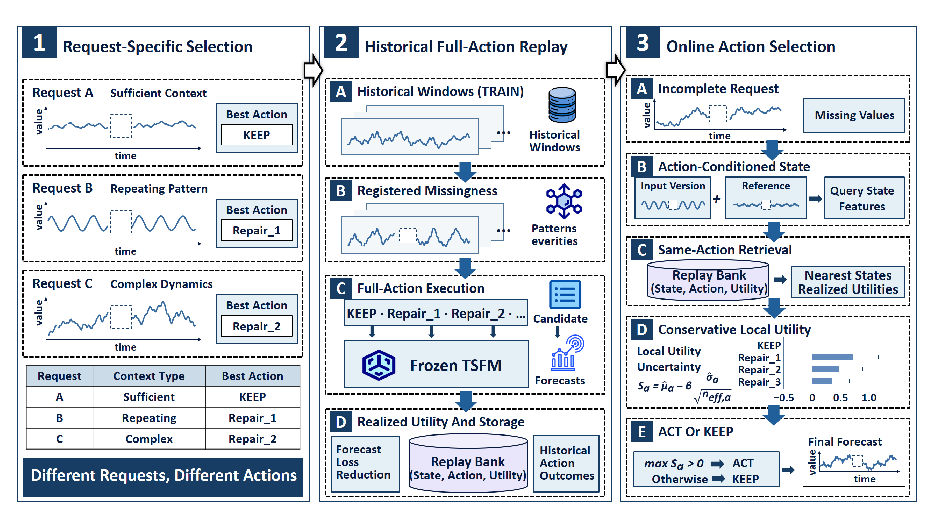
\includegraphics[width=\textwidth]{figure/fig1_example.eps}
\caption{Selective repair for incomplete forecasting requests. The left panel illustrates
  requests for which different actions may be appropriate. These examples are schematic.
  Historical replay records the forecasting utility of each admissible action. Online
  selection retrieves evidence for the current request and either executes a repair or
  retains the reference forecast.}

  \label{fig:concept}
\end{figure}

\section{Related Work}
\label{sec:related}

\subsection{Incomplete Time-Series Modeling}
\label{sec:related-incomplete}
Imputation reconstructs unavailable values using temporal or cross-channel
structure~\citep{cao2018brits,tashiro2021csdi,yoon2018gain,du2023saits,park2026t1}.
Missingness-aware forecasting instead incorporates the observation pattern into a trained
predictor~\citep{chen2024bitgraph,peng2025s4m,jang2026channeltokenformer}.
Task-oriented methods connect imputation to a downstream
objective~\citep{wang2024taskoriented,hao2025toivsf,hao2025gimcc,liang2025vida,xu2026srdi}.
Two distinctions locate the present setting against this work. On the input side, variable
subset forecasting removes entire variables at inference, whereas our requests contain gaps
inside the context. On the model side, missingness-aware forecasting requires control over
the predictor's training, whereas our predictor stays frozen. A trained imputer can therefore
supply a candidate repair here, while the decision layer determines whether that repair
should be used for the current request.

\subsection{Data-Side Adaptation for Frozen \tsfm{}s}
\label{sec:related-dataside}
TATO~\citep{qiu2026tato} shows that a frozen \tsfm{} can be adapted to heterogeneous domains
without parameter updates, by searching a transformation pipeline and selecting it from
historical task performance. Its unit of adaptation is a target domain: one pipeline serves
many requests. \introact{} makes a separate decision for each request over a fixed catalog,
using forecasting outcomes recorded for that backbone. TS-ICL~\citep{tsicl2026} is a
foundation model that natively supports imputation and partially observed look-back windows,
and it appears here only as the in-context regression backend of two catalog actions.

\subsection{Selective Decision Making}
\label{sec:related-selective}
Selective prediction trades coverage for lower
risk~\citep{chow1970optimum,vovk2005algorithmic,geifman2017selective,lei2018distribution},
and learning to defer routes a request to another decision
maker~\citep{madras2018predict,mozannar2020consistent}. \introact{} retains the same forecaster
for every request and selects whether to modify its input. Keeping the input still returns a
forecast; it is not a refusal to answer. This is a form of per-instance
algorithm selection~\citep{rice1976algorithm,xu2008satzilla}, supervised by the forecasting
utility of each repair. Executing every admissible catalog action on historical windows gives
full action feedback. Off-policy evaluation typically observes outcomes only for logged
actions~\citep{dudik2011doubly,swaminathan2015counterfactual}.
Appendix~\ref{app:ope-positioning} details the relationship. Section~\ref{sec:method}
accordingly restricts the decision object to a fixed action catalog and supervises selection
with the full action feedback recorded on historical windows.

\section{Problem Formulation and Method}
\label{sec:method}

\begin{figure}[t]
  \centering
  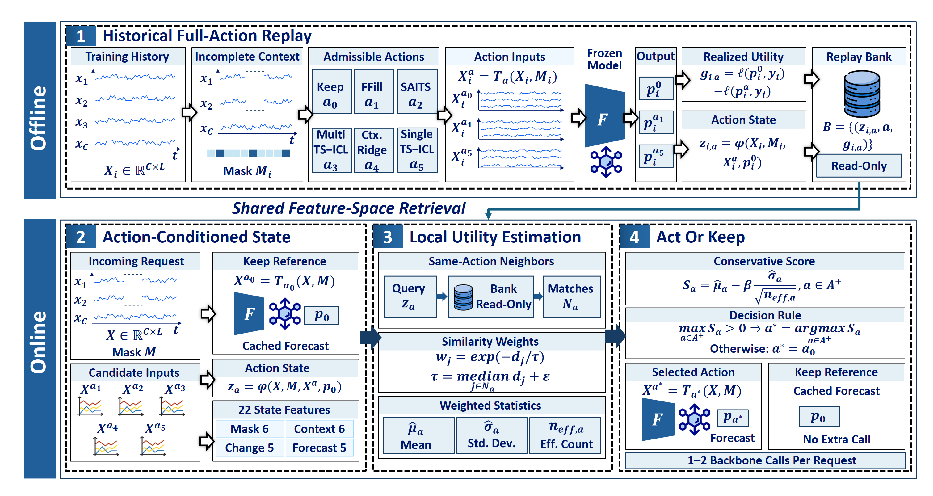
\includegraphics[width=\textwidth]{figure/fig2_Architecture.eps}
\caption{Architecture of \introact{}. Offline replay executes admissible actions on
  training windows and stores their states and realised forecasting utilities. Online
  processing forms action states from the incomplete context, candidate repairs and the
  reference forecast. Same-action retrieval supplies a local utility estimate. The decision
  returns either the forecast of the selected repair or the cached reference forecast.
  Future targets are used only for historical supervision and subsequent evaluation.}

  \label{fig:arch}
\end{figure}

\subsection{Problem Setup}
\label{sec:method-problem}
Let $X \in \mathbb{R}^{C \times L}$ denote a context with $C$ channels and length $L$,
with observation mask $M \in \{0,1\}^{C \times L}$. The future target
$Y \in \mathbb{R}^{C \times H}$ is unavailable to the decision procedure. The frozen pipeline
$F$ includes the backbone's internal preprocessing and returns $p=F(X)$. The reference action
passes the incomplete context to $F$ unchanged, so its treatment of missing values is the
backbone's own and therefore differs across backbones, as the \textsc{Keep} rows of
Table~\ref{tab:main} reflect;
the per-backbone adapter behaviour is specified in Appendix~\ref{app:method-details}.

The system may modify this input only through a fixed catalog
$\calA = \{a_0, a_1, \dots, a_J\}$ of admissible interventions, with
$J$ interventions in addition to the reference. Each action $a$ materialises an admissible
input version $X^{a} = T_a(X, M)$. The reference action $a_0$ returns the input unchanged and
corresponds to no external intervention, and $\calA^{+} = \calA \setminus \{a_0\}$ collects
the actions that modify the input. Whether a repair is worth executing is measured against
this reference. Let $\loss$ be the episode-level MASE of a forecast, which is also the primary evaluation
metric, so replay utilities and reported errors carry one scale. For a realised target
$Y$, the forecasting utility of action $a$ is the reference loss minus the repaired loss,
\begin{equation}
  g_a \;=\; \loss\!\left(F(X^{a_0}),\, Y\right) \;-\; \loss\!\left(F(X^{a}),\, Y\right),
  \label{eq:utility}
\end{equation}
so a positive $g_a$ means the repair improved the forecast relative to leaving the input
unchanged, and a negative one means it degraded it. The task is to choose
$a^\star(X, M) \in \calA$ without access to $Y$, while keeping the
number of frozen-backbone calls small.

Four constraints define the deployment protocol. No observation that has arrived and is valid
may be overwritten, so every $X^{a}$ differs from $X^{a_0}$ only at positions where $M = 0$.
A repair may write only values inside the range of the visible part of the target channel in
the context, widened by three robust
scales, and a candidate that leaves that range is recorded as unsupported instead of executed.
The bound is registered with the protocol and holds identically for the historical replay bank
of \S\ref{sec:method-replay} and for a served
request. The future target is unavailable, so no realised loss is
observable at deployment time. The reference forecast is the only forecast that may be computed
before the decision. Under this call budget, a
request may spend one forecasting-backbone call to obtain $p_0 = F(X^{a_0})$, and the forecasts
of the remaining candidates must not be inspected when the action is chosen.

\subsection{Historical Full-Action Replay}
\label{sec:method-replay}
The quantity that decides the action, $g_a$, depends on $Y$ and is not observable online, but it
is computable for a historical window whose target is already part of the available history.
Take such a window $i$, inject the registered missingness protocol to obtain $(X_i, M_i)$,
materialise every action, and execute the frozen pipeline on each version. The realised utility
of action $a$ on window $i$ is
\begin{equation}
  g_{i,a} \;=\; \loss\!\left(F(T_{a_0}(X_i, M_i)),\, y_i\right)
  \;-\; \loss\!\left(F(T_{a}(X_i, M_i)),\, y_i\right).
  \label{eq:replay-gain}
\end{equation}
Both forecasts are evaluated against the same realised future. Their loss difference records
the action's forecasting effect on that historical window.

A utility label informs a new decision only if the historical window can be matched to the
deployment request, so each outcome is stored together with a retrieval state. The state is
action conditioned:
\begin{equation}
  z_{i,a} = \phi(X_i, M_i, X_i^{a}, p_i^{0}),
  \qquad p_i^{0} = F(X_i^{a_0}),
  \qquad X_i^{a} = T_a(X_i, M_i).
  \label{eq:state}
\end{equation}
It may use the reference forecast $p_i^0$, which the
protocol already permits, and it never uses the forecast of a non-selected candidate. The
replay bank is $\calB = \{(z_{i,a}, a, g_{i,a})\}$, built once from TRAIN history and then
frozen. Deployment reads it and never writes to it.

Two properties of the bank set the scope of the method. A utility measured with one revision
of one model does not describe another, so the bank is built and held per frozen backbone
revision, and serving a new backbone family means rebuilding it. The bank also covers only the
missingness protocol registered in advance, which makes it a discrete grid over patterns and
severities.
Appendix~\ref{app:replay} reports what each restriction costs.

Using these records for a new request rests on one assumption: nearby action-conditioned
states have sufficiently similar utilities to guide selection. Section~\ref{sec:exp-ablation}
and Appendix~\ref{app:transfer} examine this assumption; the estimator itself is defined next.

\subsection{Action-Conditioned Local Utility Estimation}
\label{sec:method-scoring}
The estimator is a weighted average of the recorded utilities of the same action on nearby
states, in a fixed standardised feature space. The state $z_a$ of \eqref{eq:state} carries
twenty-two numbers in four groups: how the request is incomplete, what the observed part of the
target channel looks like, how $X^{a}$ differs from $X^{a_0}$, and what the reference forecast
$p_0 = F(X^{a_0})$ looks like. Under the present catalog, four of the five coordinates in the
third group are identically zero (Appendix~\ref{app:features}), so the varying intervention
information reduces to the fraction of positions the repair changes. Retrieval is not
restricted to a source or a horizon; the neighbourhood is meant to match on the mask geometry,
the visible context and the reference forecast. Appendix~\ref{app:features} is the canonical
list, with the window lengths and the normalisation, which is fitted on the replay bank only.

Retrieval is performed separately for each action. For action $a$, the neighbourhood
$\calN_a$ contains the $k$ bank records whose recorded action is $a$ and whose states are
closest to $z_a$ in standardised Euclidean distance. Each neighbour receives the weight
\begin{equation}
  w_i \;=\; \exp\!\left(-d_i / \tau\right),
  \qquad
  \tau \;=\; \operatorname{median}_{i \in \calN_a} d_i \;+\; \epsilon ,
  \label{eq:weights}
\end{equation}
so closer records contribute more, and the bandwidth is set by the query neighbourhood itself
rather than tuned. The constant $\epsilon$ handles zero distances. From the weighted records
the estimator computes three quantities: a local mean utility, which estimates the action's
gain for this request; a local dispersion, which measures how much the neighbouring outcomes
disagree; and an effective sample size, which measures how concentrated the weights are,
\begin{equation}
  \hat\mu_a \;=\; \frac{\sum_{i \in \calN_a} w_i\, g_{i,a}}{\sum_{i \in \calN_a} w_i},
  \qquad
  \hat\sigma_a^{2} \;=\; \frac{\sum_{i \in \calN_a} w_i\, (g_{i,a} - \hat\mu_a)^{2}}{\sum_{i \in \calN_a} w_i},
  \qquad
  n_{\mathrm{eff},a} \;=\; \frac{\left(\sum_{i \in \calN_a} w_i\right)^{2}}{\sum_{i \in \calN_a} w_i^{2}} .
  \label{eq:local-moments}
\end{equation}
The neighbourhood size $k$ and the penalty strength $\beta$ of \S\ref{sec:method-decision} are
the only searched quantities, and \S\ref{sec:method-decision} states how they are chosen. The
neighbourhood is defined by distance alone, and no threshold marks a request as outside the
replay support, so the estimator returns a value for every request it receives.
Section~\ref{sec:exp-robust} and Appendix~\ref{app:scope} treat the resulting scope as a
within-grid statement.

\subsection{Conservative Act-or-Keep Decision}
\label{sec:method-decision}
A positive local mean is not sufficient evidence for executing an action, because the
neighbourhood may be small or internally inconsistent. The decision therefore uses the
conservative score
\begin{equation}
  S_a \;=\; \hat\mu_a \;-\; \beta\, \frac{\hat\sigma_a}{\sqrt{n_{\mathrm{eff},a}}},
  \qquad a \in \calA^{+},
  \label{eq:score}
\end{equation}
where $\beta$ is a penalty strength. The action taken is
$a^{\star} = \arg\max_{a \in \calA^{+}} S_a$ when $\max_{a \in \calA^{+}} S_a > 0$, and
$a^{\star} = a_0$ otherwise.
The score is an empirical decision rule. It has no calibrated coverage or risk
guarantee~\citep{angelopoulos2024conformal}. The penalty $\beta$ is selected from a finite
grid, and the decision threshold remains zero. Because utility is defined relative to the
reference action in \eqref{eq:utility}, the zero threshold requires a positive penalised
estimate before any repair displaces \textsc{Keep}; this is a decision convention, not a
significance statement.

The two hyperparameters are selected once per backbone on the replay bank by
leave-one-parent-out cross-validation, so every bank episode is scored against a bank with all
records of its own parent removed. A parent is a non-overlapping origin window from which the
episodes are generated; Appendix~\ref{app:splits} gives the tiling rule. The grid is
$k \in \{8, 16, 32, 64, 128, 256\}$ and $\beta \in \{0, 0.5, 1, 1.64\}$, whose largest penalty
is approximately the one-sided $95\%$ normal quantile, used only as a grid value. A setting is admissible when its cross-validated
conditional harmful rate — the share of executed interventions that increase loss — stays at
or below a cap. The cap comes from the bank itself: it is
the
conditional harmful rate of the action with the highest mean realised utility there, so the
constraint says that choosing per request may not be more harmful, given that it intervenes,
than always applying the strongest single intervention. Among the admissible settings the rule
takes the lowest cross-validated source-macro MASE, and a tie on that value goes to the setting
that intervenes least. If no setting satisfies the cap, the recorded pipeline falls back to
the largest penalty strength; that fallback does not re-check the cap, so the cap is not
guaranteed on that branch, and a run in which it triggered would not meet the stated
criterion. The branch never triggered in any
recorded selection. The anchor, the cap, the admissible settings and the selected pair
are fixed for the recorded run.

The reference action is always available, so the rule always returns a forecast. It has no way
to detect that a request lies outside the replay support, so it applies to the registered
missingness grid and the results should not be read as out-of-grid generalisation.

\subsection{Deployment Procedure and Cost}
\label{sec:method-deploy}
A request is served in two stages. The first executes the reference action to obtain $p_0$,
materialises the candidate input versions and forms the states $z_a$. The second retrieves the
same-action neighbourhoods from the frozen bank, evaluates $S_a$ for every $a \in \calA^{+}$,
executes $a^{\star}$ and returns its forecast, which is the reference forecast when
$a^{\star} = a_0$.

A request costs one forecasting-backbone call for the reference action plus one more if an
intervention is executed, and the returned forecast is always one call of the unchanged $F$ on
one executed input version. Three of the five interventions build their candidate with a model
of their own, two by calling a frozen in-context imputation model and one by calling the
trained imputer, and all of that is paid before the decision.
Appendix~\ref{app:calls} keeps the one-off bank construction, candidate materialisation, the
backbone call and retrieval overhead in separate columns.

\section{Experiments}
\label{sec:exp}

\subsection{Evaluation Protocol}
\label{sec:exp-setup}
The recorded evaluation covers eight sources, ETTh1, ETTh2, ETTm1, ETTm2, Electricity,
Exchange, Traffic and Weather, with three frozen backbones. These are
Chronos-Bolt~\citep{chronosbolt2025}, TimesFM-2.5~\citep{das2024timesfm} and
Chronos-2~\citep{chronos2_2025}. A separate replay bank is built for each backbone using the
same selection procedure. Context length is $L=512$, with horizons $H \in \{96,192\}$.
The main comparison uses $10\%$ missingness across four deterministic patterns.
Additional evaluations use $30\%$ and $50\%$ missingness without retuning.
Appendix~\ref{app:data-protocol} defines the masks and metrics.

The catalog contains \textsc{Keep} and five repairs. Each comparison partner answers a
different question about the decision. The unchanged input asks whether external repair is
needed at all. The best fixed repair, selected on TRAIN, asks whether the choice must be made
per request. R2-CART, a simple selector over the same state features, asks what the more
elaborate estimation adds. Fixed SAITS supplies a strong single-repair reference, and a TATO
adaptation covers domain-level pipeline selection. Appendix~\ref{app:baseline-config}
specifies their implementations. The catalog oracle uses future targets and serves only as a
diagnostic.

Each source is split chronologically with an $L+H$ purge. TRAIN is partitioned into the
replay bank and an internal evaluation block. The reported evaluation contains 95 parents
and 760 episodes per backbone at each severity. MASE is aggregated equally across sources,
with RMSSE as a secondary metric. Recorded paired bootstrap intervals use parents as clusters.
Appendix~\ref{app:splits} specifies the partitions and Appendix~\ref{app:metric-conventions}
defines aggregation.

The current design incorporates observations from earlier evaluations on this TEST block,
including Chronos-2. Consequently, the reported comparisons are post-hoc and Chronos-2 is
an additional backbone comparison. Neither repeated evaluation on this block nor the reported
bootstrap intervals provide a new independent confirmation.

\subsection{Variation in Repair Utility}
\label{sec:exp-exists}
The recorded diagnostics show that no single action is best for every request.
Figure~\ref{fig:utility} reports oracle-best shares across the catalog actions, from
$11.1\%$ to $24.8\%$, with
\textsc{Keep} best on $19.3\%$ of episodes. The catalog oracle reaches 1.258 source-macro
MASE compared with 1.576 for \textsc{Keep}, indicating room for better action selection.
Each repair both helps and harms individual forecasts.
Appendix~\ref{app:opportunity} breaks the same episodes down by how much improvement was
available. These observations establish that potential gains from request-specific selection
exist; they do not by themselves show that a deployable rule can realise them.

Reconstruction quality provides limited guidance for this decision. On the recorded Bolt
episodes, the repair with the
lowest reconstruction error also has the highest forecasting utility on $19.3\%$ of episodes
(a value that coincidentally matches the \textsc{Keep} best share above).
The rankings disagree on $44.5\%$ of ordered pairs, with mean within-episode Spearman
correlation of 0.12. These statistics compare actions within the same episode, avoiding
cross-source scale differences. Appendix~\ref{app:recutils} reports the full comparison.

\begin{figure}[t]
\centering

\includegraphics[width=\textwidth]{figure/fig3_action_utility.eps}
\caption{Action-dependent forecasting utility. (a) Oracle-best frequency and the share of available episodes improved by each repair. The beneficial share is undefined for KEEP. (b) Mean realised utility relative to KEEP, shown in units of $10^{-2}$. Single and Multi denote the two TS-ICL actions. Exact values and action availability are reported in Table~\ref{tab:heterogeneity}.}
\label{fig:utility}
\end{figure}

Together, the two diagnostics motivate supervising selection with forecasting utility rather
than reconstruction quality. The remaining question is whether a deployable decision rule can
turn the observed variation into better forecasts, which the next section examines.

\subsection{Forecasting Performance}
\label{sec:exp-main}
Table~\ref{tab:main} compares the methods at $10\%$ missingness.
\introact{} reaches 1.437 source-macro MASE, compared with 1.576 for \textsc{Keep}, 1.488
for Best Fixed and 1.458 for R2-CART. Fixed SAITS reaches 1.459 and TATO reaches 1.616.
The lowest deployable MASE is achieved by \introact{} on Bolt and Chronos-2, and by fixed
SAITS on TimesFM. Thus, the aggregate advantage does not imply a win on every backbone.

Paired differences against \textsc{Keep} are $-0.0881$ on Bolt, $-0.1283$ on TimesFM and
$-0.2014$ on Chronos-2. Their recorded $95\%$ intervals are respectively
$[-0.1530,-0.0256]$, $[-0.2018,-0.0543]$ and $[-0.2876,-0.1180]$.
All exclude zero. The intervals against Best Fixed and R2-CART include zero, so these
comparisons do not establish an accuracy advantage over either control. Holm-adjusted
comparisons against \textsc{Keep} remain below $0.05$ on each backbone, subject to the
post-hoc evaluation boundary stated above.

The method also has the lowest mean rank among the six deployable methods on each backbone.
Rank is a descriptive summary and does not establish consistent improvement in every cell.
The TATO result applies to the adaptation and search budget specified in
Appendix~\ref{app:baseline-config}. Per-source results appear in Appendix~\ref{app:datasets},
and costs are reported in Appendix~\ref{app:calls}.

\begin{table}[t]
  \caption{Main comparison on TEST at $10\%$ missingness, source-macro averaged, lower is
  better everywhere. \best{Bold} is the best value of a column and \second{underline} the
  second. Average rank ranks the deployable methods per request (competition ranking, ties
  within $10^{-12}$ share the better rank, requests where a method has no finite value are
  excluded for that method), averaged over the 760 requests of each backbone and then over
  backbones. The oracle
  reads the future target and is excluded from every rank. Each backbone uses its own TRAIN replay bank. These are post-hoc comparisons. Table~\ref{tab:app-roster} defines the rows.}
  \label{tab:main}
  \centering
  \small
  \setlength{\tabcolsep}{3.5pt}
\adjustbox{max width=\textwidth}{\begin{tabular}{lccccc}
    \toprule
    Method & Bolt & TimesFM & Chronos-2 & Overall MASE & Avg.\ rank \\
    \midrule
Native KEEP & 1.466 & 1.682 & 1.579 & 1.576 & 3.36 \\
Best Fixed & 1.428 & 1.579 & 1.456 & 1.488 & \second{2.94} \\
R2-CART & \second{1.402} & 1.588 & \second{1.385} & \second{1.458} & 2.97 \\
Fixed SAITS & 1.469 & \best{1.465} & 1.441 & 1.459 & 2.98 \\
TATO & 1.620 & 1.614 & 1.614 & 1.616 & 4.10 \\
    \midrule
\rowcolor{bestgray}\introact{} & \best{1.378} & \second{1.554} & \best{1.378} & \best{1.437} & \best{2.79} \\
    \midrule
Catalog Oracle & \oracle{1.234} & \oracle{1.315} & \oracle{1.226} & \oracle{1.258} & \oracle{n/a} \\
    \bottomrule
  \end{tabular}}
\end{table}

Two source-level diagnostics locate where this advantage comes from. The first asks whether
the gain comes from identifying which repair suits a source rather than which repair suits a
request. A source-level fixed policy applies, per source, the single action with the highest
mean realised utility on the replay bank, with \textsc{Keep} as the registered fallback where
that action is unsupported, all fixed on TRAIN. It reaches 1.360, 1.527 and 1.448 source-macro
MASE: better than the full rule on Bolt ($+0.0181$, $[0.0061,0.0296]$) and TimesFM
($+0.0269$, $[0.0035,0.0526]$), worse on Chronos-2 ($-0.0704$, interval includes zero), and
close in aggregate (1.445 against 1.437). Request-level selection therefore does not
outperform a per-source fixed choice on two of the three backbones.

The second diagnostic recomputes the source-macro paired differences on each seven-source
subset of TEST. The margins over the unchanged input and over TATO keep their sign on every
subset of every backbone. The margins over the stronger controls do not: removing Exchange
reduces the paired difference against Best Fixed from $-0.0497$ to $-0.0061$ on Bolt and
reverses it on TimesFM and Chronos-2 ($+0.0095$ and $+0.0073$), and the same concentration
appears against the simple selector. The aggregate advantage over Best Fixed and R2-CART
therefore rests largely on one source, while the advantage over the unchanged input is
broad-based. Appendix~\ref{app:source-diagnostics} reports the full tables.

Average error also does not distinguish repairs that help from repairs that harm, so the next
section examines how often the method intervenes and what the executed interventions cost.

\subsection{Intervention Frequency and Harm}
\label{sec:exp-harm}
At the default operating point, \introact{} intervenes on $65.4\%$ of requests, of which
$40.2\%$ increase loss. Its harmful loss — the loss increase accumulated by executed harmful
interventions, averaged over all requests (Appendix~\ref{app:diagnostic-conventions}) — is
0.0375, compared with 0.0513 for Best Fixed and
0.0584 for R2-CART. Figure~\ref{fig:harm} retains these aggregate diagnostics in the appendix.

The lower harm could in principle come from intervening less often rather than from choosing
better requests, so the evaluation includes controls that intervene at a comparable
frequency. Three distinct designs answer three distinct questions and are reported
separately. Random gating keeps the full rule's recommended repair and randomises only
whether it is executed. The mean-only and linear controls keep their own scoring rules but
recalibrate an acceptance threshold. A random-\textsc{Keep} variant of Best Fixed keeps the
fixed repair and randomises whether it is executed. All thresholds and probabilities are
calibrated on the development block to the full method's development intervention rate and
then frozen; development matching does not guarantee equal TEST frequencies, so
Figure~\ref{fig:gate-controls} reports the actual TEST rates alongside accuracy and harm.

Against random gating, the full rule improves MASE by 0.0292, 0.1182 and 0.0682 on Bolt,
TimesFM and Chronos-2, and all three nominal intervals exclude zero. Its advantage over the
mean-only control excludes zero only on TimesFM, and over the linear control only on Bolt;
those two controls also change which repair is recommended, so they do not isolate the
acceptance decision. Random gating uses a single recorded seed and nevertheless has lower
harmful loss than the full rule on all three backbones. Against the frequency-matched
partners, the random-\textsc{Keep} fixed policy is worse than the full rule on all three
backbones ($-0.0640$, $-0.0852$ and $-0.1183$, every nominal interval excluding zero), at
realised TEST rates of $52.2\%$, $33.7\%$ and $49.6\%$ — below the development targets,
because the fixed repair is unsupported on part of the requests and the rate is not
rematched. The threshold-matched simple selector reaches 1.404, 1.590 and 1.412
source-macro MASE, and its paired difference against the full rule excludes zero only on
Bolt ($-0.0252$, $[-0.0495,-0.0011]$). Appendices~\ref{app:gate-controls}
and~\ref{app:matched-partners} record the exact values and the limitations of these post-hoc
comparisons.

These comparisons bound rather than isolate the mechanism. Intervening less often does not
by itself reproduce the full rule's accuracy, and the margin over the frequency-matched
simple selector remains backbone-dependent. What the controls jointly support is an
accuracy--harm tradeoff: the full rule converts its interventions into lower error more
effectively than frequency-matched alternatives, while harmful loss stays above that of
random gating on every backbone.

\begin{figure}[t]
\centering
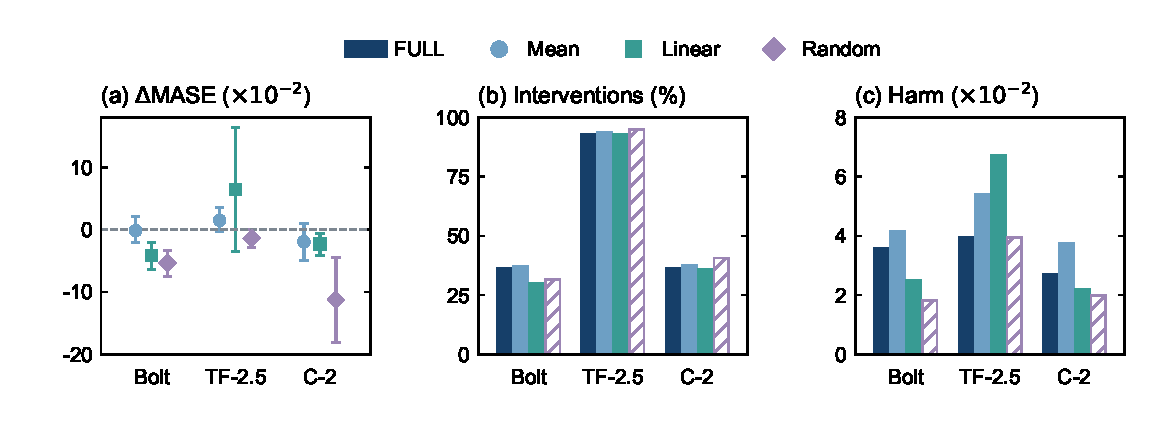
\includegraphics[width=\textwidth]{figure/fig7_gate_controls.eps}
\caption{Gate controls calibrated on the development block and frozen for TEST.
(a) FULL minus each control in MASE, with nominal $95\%$ parent-bootstrap intervals.
Negative values favour FULL. (b) Actual TEST intervention frequency. (c) Harmful loss.
TF-2.5 denotes TimesFM-2.5 and C-2 denotes Chronos-2. Development frequency matching does not guarantee
equal TEST frequencies. Random gating uses seed 101.}
\label{fig:gate-controls}
\end{figure}

\subsection{Effects of Utility Estimation and State Representation}
\label{sec:exp-ablation}
Table~\ref{tab:ablation} varies how the selector uses historical utility. A1 replaces the
local estimate with action-wise global means. A2-M pools local neighbours across repair
actions and retains only global action-specific priors. A5 predicts utility linearly from the
same state. All three reuse the full method's frozen $(k,\beta)$ without retuning. Global
means intervene on every request and reach 1.475 aggregate MASE with the highest harmful loss
in the table (0.0697), so a per-action global summary does not by itself protect accuracy.
Pooling
action utilities increases MASE from 1.4366 to 1.4470 and intervention frequency from
$65.4\%$ to $82.6\%$; the paired difference is $-0.0252$ on Bolt, with a nominal $95\%$
interval of $[-0.0478,-0.0025]$, and the intervals include zero on TimesFM and Chronos-2.
The linear estimator reaches 1.4343. Pooling also changes the balance between local evidence
and global priors, so it is not a single-factor ablation; within the tested design, the
comparisons support action-specific local estimation without establishing that the local
estimator outperforms linear prediction. On the decision side, always acting (A4) raises
harmful loss from 0.0375 to 0.0533, which is the recorded cost of removing the \textsc{Keep}
branch.

A second group varies the state. A3 removes the reference-forecast features and reaches
1.446, close to the full method. A2-F removes the five intervention features under the same
frozen configuration and improves aggregate MASE to 1.4185, with the Bolt interval favouring
the reduced state. Four of those five features are identically zero under the present catalog
(Appendix~\ref{app:features}), so A2-F effectively removes one varying coordinate together
with the selection the feature group induces; its favourable error is retained as recorded,
not relabelled as evidence against the mechanism. Appendix~\ref{app:estimation-analyses}
records both controls with per-backbone intervals.

A2-F is a fixed-configuration ablation: it answers what the feature group contributes when
nothing else changes. A different comparison asks whether the reduced representation should
replace the full one, which requires its own parameters. Given its own TRAIN-side selection
under the identical grid, cap and cross-validation, the reduced 17-dimensional state picks
weaker penalties everywhere. On the development block it degrades TimesFM
(MASE $1.0952 \to 1.1182$, paired interval
$[0.0012,0.0581]$ for the increase, harmful loss $0.0111 \to 0.0351$, intervention rate
$46.7\% \to 81.6\%$), leaves Bolt's accuracy unchanged while raising its harmful loss, and
improves Chronos-2 ($1.1365 \to 1.1131$, interval $[0.0035,0.0477]$ for the decrease). Under the revision cycle's adoption rule — adopt
only if development error falls without raising harm and without a single-backbone
regression — the mixed evidence keeps the full 22-dimensional state. The retuned reduced
state's TEST aggregate (1.4280 against 1.4366) is recorded for the record only, and the
selection and evaluation tables appear in Appendix~\ref{app:compact-selection}.

\begin{table}[t]
  \caption{Core ablation and cost at $10\%$ severity. Every row reads the same catalog
  prediction cache, so the rows differ only in how the stored utilities are summarised and
  thresholded. Calls counts forecasting-backbone calls per request. Candidate materialisation
  is reported separately in Appendix~\ref{app:calls}.}
  \label{tab:ablation}
  \centering
  \small
  \setlength{\tabcolsep}{3.5pt}
\adjustbox{max width=\textwidth}{\begin{tabular}{lccccc}
    \toprule
    Variant & MASE $\downarrow$ & Intervention rate & Conditional HIR $\downarrow$ & Harmful loss $\downarrow$ & Calls $\downarrow$ \\
    \midrule
    Full \introact{}          & 1.437   & 65.4\%   & 40.2\%   & 0.0375   & 1.65 \\
    A1 Global utility          & 1.475     & 100.0\%     & 43.9\%     & 0.0697     & 2.00 \\
    A2-M Pooled action utilities & 1.447 & 82.6\% & 44.4\% & 0.0478 & 1.83 \\
    A3 w/o reference-forecast state & 1.446 & 67.4\%     & 40.4\%     & 0.0419     & 1.67 \\
    A4 Always act              & 1.447     & 100.0\%     & 42.1\%     & 0.0533     & 2.00 \\
    A5 Parametric utility predictor & 1.434 & 86.7\%    & 43.7\%     & 0.0549     & 1.87 \\
    \midrule
    \bottomrule
  \end{tabular}}
\end{table}

\subsection{Sensitivity to Missingness and Replay Support}
\label{sec:exp-robust}
The main comparison covers one primary severity, so the evaluation extends to the other
registered levels and patterns. Figure~\ref{fig:robust} compares the same configurations at
three registered severities.
\introact{} has lower MASE than \textsc{Keep} at each level. Its values are 1.437, 1.698
and 1.735, compared with 1.576, 1.794 and 1.875 for the unchanged input. R2-CART reaches
1.678 and 1.721 at the two higher severities, so the default method does not retain the
lowest aggregate error throughout the sweep. All three severities occur in replay
construction, so the sweep measures performance within the sampled missingness grid, and
each backbone uses a bank constructed with its own forecasts.
Appendices~\ref{app:severity-full} and \ref{app:pattern} report the complete breakdowns.

The method also depends on the replay bank as its source of historical support, and three
recorded checks vary that support in different ways. Subsampling the bank asks how much
history the selection needs (Appendix~\ref{app:replaysize}). Repeating the TRAIN-side
selection under bank subsamples asks how stable the chosen $(k,\beta)$ is
(Appendix~\ref{app:selstability}). Regenerating the missingness masks of the same parents
asks how much the result depends on the particular mask realisation
(Appendix~\ref{app:seeds}). These checks vary the historical support, the selected
configuration and the mask realisation of the same parents respectively; none of them is an
independent generalisation test.

\begin{figure}[t]
  \centering
  
\includegraphics[width=\textwidth]{figure/fig5_missingness_severity.eps}
  \caption{Forecasting error across registered missingness severities and the largest degradation relative to KEEP in any pattern, backbone and severity cell. Each point reproduces the source-macro MASE averaged over three backbones, two horizons and four patterns. Configurations are unchanged across levels. All three levels occur in replay construction. Full numerical results are retained in Appendix~\ref{app:severity-full}.}
  \label{fig:robust}
\end{figure}

\subsection{Deployment Cost}
\label{sec:exp-cost}
Serving follows the two-stage order of \S\ref{sec:method-deploy}, and the recorded costs are
kept by component. The full method averages 1.65 forecasting-backbone calls per request: one
reference call, plus one for the selected repair when an intervention executes. Candidate
construction is paid before selection, and three of the five repairs build their candidate
with a model of their own. Retrieval and scoring add overhead measured separately from the
backbone calls, and the one-off bank construction is a cold-start cost.
Appendix~\ref{app:calls} reports the measured call counts, the failure audit and a synthetic
latency accounting; end-to-end request latency has not been measured under this
configuration, so no latency quantiles are claimed. These figures answer one question: which
computations per-request selection adds beyond the reference forecast.

\newpage
\section{Conclusion}
\label{sec:conclusion}
We studied whether and how an incomplete context should be repaired before forecasting with
a frozen model, treating the unchanged input as an explicit option. \introact{} turns
historical action outcomes into forecasting-utility supervision and combines action-specific
local estimates with a dispersion penalty to decide whether to intervene. The recorded
evaluation shows broad-based improvement over the unchanged input, while the advantage over
the stronger simple policies is concentrated in one source, a per-source fixed choice is at
least as accurate on two of the three backbones, and lower error coexists with higher harmful
loss than random gating — an accuracy--harm tradeoff rather than a uniform win. Because
earlier test observations informed the design, independent evaluation remains necessary,
together with tests on naturally missing data and requests outside the replay grid.
\label{sec:main-end}

\section*{AI Use Statement}
\label{sec:ai-statement}
The authors used ChatGPT to assist with English language polishing, including the
Introduction and Related Work sections, literature search and reference checking.
Generative AI tools also assisted with code preparation and the production of figures
from recorded experimental data. All AI-assisted content was carefully reviewed,
substantively edited, and verified by the authors, who take full responsibility for
the final content and scientific validity of the publication. The numerical tables
and figures retain the recorded experimental results.

\subsubsection*{Ethics statement}
This work studies input governance for frozen forecasting models on public benchmark datasets.
It does not involve human subjects, personal data, or deployment decisions with direct
societal consequences. We impose an integrity constraint under which an admissible
intervention cannot overwrite an observation that is marked as valid and available, because
silently replacing a real measurement would be a data integrity problem regardless of its
forecasting effect. We do not claim safety, robustness, or generality beyond the measured
conditions.

\subsubsection*{Reproducibility statement}
We provide the complete experimental protocol, the final TRAIN and TEST split with the
purging rule, the missingness generation procedure, the intervention catalog, the state
feature definitions, the hyperparameter search spaces, the failure policy, and the statistical
analysis in Appendix~\ref{app:data-protocol} and Appendix~\ref{app:splits}.
Appendix~\ref{app:reprodetails} specifies the result-record schema and the traceability checks.
All reported tables are generated from retained raw predictions and versioned configurations.

\bibliography{references}
\bibliographystyle{iclr2027_conference}

\appendix

\newpage

\section*{Appendix map}
\label{app:map}
Table~\ref{tab:app-map} lists what each appendix section contains. The appendix is organised
by the question each part answers.

\begin{table}[htbp]
  \caption{Appendix map. Sections are lettered in order of appearance.}
  \label{tab:app-map}
  \centering
  \small
  \setlength{\tabcolsep}{4pt}
\adjustbox{max width=\textwidth}{\begin{tabular}{@{}p{.18\textwidth}p{.44\textwidth}p{.31\textwidth}@{}}
    \toprule
    Section & Contents & Question it answers \\
    \midrule
    A. Evaluation protocol & scope and assumptions, the TRAIN and TEST split with purging, the dataset and missingness protocol, baseline availability and configuration & what exactly was fixed before the evaluation ran? \\
    B. Method and implementation details & the intervention catalog, the state features, the off-policy positioning, replay construction, local utility estimation, the complete-input contract & how is the method defined, exactly as implemented? \\
    C. Forecasting results & action-utility values, reconstruction versus forecasting utility, per-source and per-pattern tables, the source-level fixed policy and leave-one-source-out & does the aggregate hold action by action, source by source, and pattern by pattern? \\
    D. Intervention frequency and harm & governance diagnostics, opportunity strata, gate controls, frequency-matched comparison partners & how often does each rule intervene, and is the full rule's frequency what carries its result? \\
    E. Estimation and state analyses & the full ablation vector, the mechanism and feature controls, the reduced-state selection check & which component carries the gain, and does the state representation survive its own selection? \\
    F. Sensitivity analyses & the severity sweep, replay-bank size, selection stability, mask-realisation stability & does the result rest on one severity, one bank size, one configuration, or one mask? \\
    G. Cost and reproducibility & the runtime and failure audit, the result-record schema and anchors, the development negative results & what does a request cost, and can every reported number be traced back to a stored artefact? \\
    \bottomrule
  \end{tabular}}
\end{table}

\begin{figure}[t]
\centering

\includegraphics[width=\textwidth]{figure/fig4_intervention_harm.eps}
\caption{Intervention risk at $10\%$ missingness. Panel (a) reports harmful loss. Panel (b) compares intervention frequency with the harmful rate among executed interventions, shown by filled and hatched bars, respectively. KEEP never intervenes, so its conditional harmful rate is undefined. Fixed denotes Best Fixed, CART denotes R2-CART, and Ours denotes IntroAct-TS. Values are descriptive aggregates over the three backbones.}
\label{fig:harm}
\end{figure}

\section{Evaluation Protocol}
\label{app:protocol}

This section fixes everything that was registered before the evaluation ran, and it
supports \S\ref{sec:exp-setup}.

\subsection{Scope and Assumptions}
\label{app:scope}
The replay bank samples four missingness patterns and three severities on the registered
sources. The estimator returns a score even when a request differs from this support, since
retrieval has no explicit support threshold. Results therefore apply to the sampled grid.
They do not establish performance on naturally missing streams or new missingness mechanisms.

The catalog and backbone revision are fixed. Changing the revision requires rebuilding the
bank because each utility belongs to the model that produced it. Selection stability is
examined through parent-level bank subsampling in Appendix~\ref{app:selstability}.
Table~\ref{tab:app-claims} summarises the scope of these measurements.

\begin{table}[htbp]
  \caption{What the evidence supports and what it does not. The scope follows from the evaluation protocol and the empirical decision rule.}
  \label{tab:app-claims}
  \centering
  \small
  \setlength{\tabcolsep}{4pt}
\begin{tabular}{@{}p{0.46\textwidth} p{0.46\textwidth}@{}}
    \toprule
    Supported by the reported evidence & Not claimed anywhere \\
    \midrule
    Selective intervention inside the registered missingness grid, on the four patterns and three severities that were replayed & out-of-grid or out-of-distribution missingness generalisation \\
    Application of the same procedure to three backbones, each with a separate replay bank, in a post-hoc comparison & that the method can detect that its historical evidence is insufficient for the request in front of it \\
    A conservative score that orders actions and a threshold that decides whether any of them runs & any coverage or risk-control guarantee for that score \\
    Behaviour under controlled deletion from complete series & that the results extend to naturally incomplete deployment streams \\
    A broad-based margin over the unchanged input, and over random intervention at matched frequency & a uniform accuracy advantage over the stronger simple controls on every source or backbone \\
    \bottomrule
  \end{tabular}
\end{table}

\subsection{Splits, Purging, and the Final Evaluation Set}
\label{app:splits}
Each source is split chronologically into TRAIN and TEST with an $L+H$ purge.
The replay bank, feature normalisation and fitted selectors use TRAIN. Earlier results on
the same TEST block informed the current method design. The split separates fitting data
from evaluation data, while the present comparison remains post-hoc.

TRAIN is then partitioned at the parent level. Within each source the admissible TRAIN parents
are sorted by origin time and split at $80/20$ into the replay bank and TRAIN-eval. The bank is
the only evidence the method reads, and it is also where $k$ and $\beta$ are chosen by
leave-one-parent-out cross-validation, so no separate selection block is held out for them.
TRAIN-eval is the internal acceptance check run once before the configuration is frozen, and
it is not an evaluation set for any reported number. Parents tile at $L + \max(H)$, so two
parents never share a raw row, and the gap between the last TRAIN window and the first TEST
window exceeds the purge on every source.
Table~\ref{tab:app-splits} records the realised sizes, including the TEST block.
Four further recorded blocks serve secondary analyses and select nothing: TEST-30 and
TEST-50 repeat the TEST parents at $30\%$ and $50\%$ severity
(Appendix~\ref{app:severity-full}), and TEST-M2 and TEST-M3 repeat them under two further
deterministic mask realisations (Appendix~\ref{app:seeds}). Two historical blocks of the
development line, a hash-sampled-severity bank variant and a second mask-seed bank, are
retained in the repository but enter no number in this paper.

\begin{table}[htbp]
  \caption{Realised split sizes. Counts are of admissible parents and not of correlated mask
  variants, so a parent with several patterns or severities still contributes one unit to
  every statistic in the paper. TEST is the evaluation population for every table in the main
  text, and it is disjoint from both TRAIN blocks.}
  \label{tab:app-splits}
  \centering
  \small
  \setlength{\tabcolsep}{4pt}
\adjustbox{max width=\textwidth}{\begin{tabular}{@{}p{.14\textwidth}rrrp{.42\textwidth}@{}}
    \toprule
    Split & Parents & Episodes & Sources covered & Used for \\
    \midrule
    Replay bank  & 223   & 5352   & 8   & replay bank, feature normalisation, baseline training, selection of $k$ and $\beta$ by cross-validation \\
    TRAIN-eval   & 53  & 424  & 8  & frozen-configuration acceptance check \\
    \midrule
    TEST         & 95  & 760  & 8  & post-hoc evaluation in the main text \\
    \bottomrule
  \end{tabular}}
\end{table}

\subsection{Dataset and Missingness Protocol}
\label{app:data-protocol}
The missingness mechanism is frozen before any method is run, and every mask is derived
deterministically from a key that identifies the parent and the pattern. This subsection fixes
the four patterns, the derivation rule, and the metric conventions that depend on the data.

\subsubsection{Missingness Patterns}
\label{app:patterns}
Table~\ref{tab:app-patterns} defines the four deterministic patterns. Every mask is derived
by a deterministic hash of
\texttt{source + parent + origin + horizon + pattern + protocol\_seed} and is never moved
after forecasts are seen. The severity of an episode is not drawn from this key: the replay
bank enumerates all three registered severities $\{10\%, 30\%, 50\%\}$ on every parent,
pattern and horizon, and the severity only sets the deletion budget of the mask.

\begin{table}[htbp]
  \caption{The four registered missingness patterns. All four are applied to the same parents,
  so pattern effects are measured on a common parent set rather than on different subsets of
  the data.}
  \label{tab:app-patterns}
  \centering
  \small
  \setlength{\tabcolsep}{4pt}
\begin{tabular}{@{}l p{0.34\textwidth} p{0.40\textwidth}@{}}
    \toprule
    Pattern & What is removed & Why it is included \\
    \midrule
    P1 point missing    & scattered single positions & the classical random-missing regime \\
    P2 target block     & a contiguous block on the target variable & a sensor outage on the variable being forecast \\
    P3 shared block     & several visible variables over the same interval & a channel or acquisition outage affecting the whole panel \\
    P4 tail missing     & a block adjacent to the forecast origin & observations that have not arrived yet at request time \\
    \bottomrule
  \end{tabular}
\end{table}

\subsubsection{Metric Conventions}
\label{app:metric-conventions}
The statistical unit is the parent. Paired cluster bootstrap with 2,000 resamples
over parent blocks gives 95\% confidence intervals on source-macro MASE differences against
each baseline, the source-macro aggregation is applied inside every resample, and Holm
correction~\citep{holm1979simple} is applied across the pre-declared baseline comparisons.
The family is the five comparisons of \introact{} against the deployable baselines on one
backbone, and the ablations stay outside it because they are variants of this method rather
than competing claims. Table~\ref{tab:app-holm} lists every raw and adjusted value.
Average rank and won cells are descriptive summaries only, and the headline claim rests on
paired differences with confidence intervals.

\begin{table}[htbp]
  \caption{Paired differences against the deployable baselines with the Holm adjustment.
  A negative difference favours \introact{}. The p-value is two sided and read off the same
  bootstrap draws as the interval, so it cannot fall below one over the number of resamples.}
  \label{tab:app-holm}
  \centering
  \small
  \setlength{\tabcolsep}{4pt}
\adjustbox{max width=\textwidth}{\begin{tabular}{llcccc}
    \toprule
    Backbone & Comparison & Difference & 95\% interval & $p$ & $p$ after Holm \\
    \midrule
    Bolt & the untouched input & -0.0881 & [-0.1530, -0.0256] & 0.0010 & 0.0040 \\
    Bolt & the best fixed intervention & -0.0497 & [-0.1008, +0.0013] & 0.0730 & 0.1830 \\
    Bolt & the simple selector & -0.0239 & [-0.0495, +0.0008] & 0.0610 & 0.1830 \\
    Bolt & the fixed imputer & -0.0908 & [-0.2201, +0.0347] & 0.3220 & 0.3220 \\
    Bolt & TATO & -0.2418 & [-0.3397, -0.1558] & 0.0005 & 0.0025 \\
    TimesFM & the untouched input & -0.1283 & [-0.2018, -0.0543] & 0.0005 & 0.0025 \\
    TimesFM & the best fixed intervention & -0.0249 & [-0.0700, +0.0202] & 0.3430 & 1.0000 \\
    TimesFM & the simple selector & -0.0348 & [-0.0912, +0.0214] & 0.4130 & 1.0000 \\
    TimesFM & the fixed imputer & +0.0884 & [-0.0352, +0.2140] & 0.4560 & 1.0000 \\
    TimesFM & TATO & -0.0602 & [-0.2607, +0.1342] & 0.5600 & 1.0000 \\
    Chronos-2 & the untouched input & -0.2014 & [-0.2876, -0.1180] & 0.0005 & 0.0025 \\
    Chronos-2 & the best fixed intervention & -0.0785 & [-0.1665, +0.0077] & 0.1600 & 0.3200 \\
    Chronos-2 & the simple selector & -0.0067 & [-0.0436, +0.0318] & 0.7170 & 0.7170 \\
    Chronos-2 & the fixed imputer & -0.0631 & [-0.1140, -0.0121] & 0.0040 & 0.0120 \\
    Chronos-2 & TATO & -0.2365 & [-0.3348, -0.1469] & 0.0005 & 0.0025 \\
    \bottomrule
  \end{tabular}}
\end{table}

Mask variants of the same parent are never
treated as independent samples, and pattern, severity, and backbone breakdowns are secondary
analyses without cell-by-cell significance testing.

MASE~\citep{hyndman2006mase} is the primary metric and RMSSE is the secondary metric. Both
scale the error of a source by its own seasonal naive error, computed on the TRAIN portion of
that source and therefore never on the evaluation block. With $y_t$ the target channel and $m$
the registered seasonal period of the source,
\begin{equation}
  \mathrm{MASE} = \frac{\mathrm{MAE}}{\frac{1}{T-m}\sum_{t} \lvert y_t - y_{t-m} \rvert},
  \qquad
  \mathrm{RMSSE} = \sqrt{\frac{\mathrm{MSE}}{\frac{1}{T-m}\sum_{t} (y_t - y_{t-m})^2}},
  \label{eq:metrics}
\end{equation}
so the two metrics share the same seasonal naive difference series but not the same power of
it, and RMSSE is not the square root of MASE. The scaling constants are computed per channel
before any aggregation over channels, and the registered periods are listed in
Table~\ref{tab:app-seasonality}. A degenerate seasonal naive error, meaning a constant or
all-missing TRAIN series, leaves the metric undefined and is reported as unavailable. Aggregation is source-macro, first over parents within a source and then equally over
the eight sources, and the same order is applied inside every bootstrap resample. MAE and RMSE
are reported per source and are never averaged across sources, because the sources have
different scales and a cross-source average of a raw error has no common unit.

\begin{table}[htbp]
  \caption{Per-source seasonal periods and context conventions used by the metric
  denominators. Context length is $L = 512$ for every source. The seasonal period is the
  sampling-frequency period registered before any run, not a tuned quantity.}
  \label{tab:app-seasonality}
  \centering
  \small
  \setlength{\tabcolsep}{4pt}
\adjustbox{max width=\textwidth}{\begin{tabular}{lccc}
    \toprule
    Source & Seasonal period $m$ & Channels & Scaling \\
    \midrule
    ETTh1 / ETTh2 & 24 & 7 & TRAIN seasonal naive error of the target channel \\
    ETTm1 / ETTm2 & 96 & 7 & TRAIN seasonal naive error of the target channel \\
    Electricity & 24 & 321 & TRAIN seasonal naive error of the target channel \\
    Exchange & 5 & 8 & TRAIN seasonal naive error of the target channel \\
    Traffic & 24 & 862 & TRAIN seasonal naive error of the target channel \\
    Weather & 144 & 21 & TRAIN seasonal naive error of the target channel \\
    \bottomrule
  \end{tabular}}
\end{table}

\subsubsection{Diagnostic Conventions}
\label{app:diagnostic-conventions}
The diagnostics require explicit counting conventions, and
Table~\ref{tab:app-counting} specifies the rules used for the recorded evaluation.

\begin{table}[htbp]
  \caption{The four counting rules used for the recorded evaluation. Each one is a
  counting convention, and a different convention would change a reported number
  without changing a single forecast.}
  \label{tab:app-counting}
  \centering
  \small
  \setlength{\tabcolsep}{4pt}
\begin{tabular}{@{}p{0.17\textwidth} p{0.40\textwidth} p{0.33\textwidth}@{}}
    \toprule
    Quantity & Rule & Boundary case \\
    \midrule
    Oracle-best action & the admissible action with the smallest realised loss & ties go to the first action in the frozen catalog order, so the shares sum to one. Unsupported, aliased and failed actions are excluded from the argmin \\
    Utility sign & harmful when $g_{i,a} < 0$ strictly, beneficial when $g_{i,a} > 0$ strictly & $g_{i,a} = 0$ enters neither rate and is reported as its own count \\
    Beneficial precision & executed interventions with strictly positive utility, over executed interventions & undefined when nothing was executed, and reported as unavailable \\
    Opportunity strata & two pre-declared quantiles of $\Delta_i$ on the replay bank, applied unchanged to TEST & the same two values partition every method and no boundary is recomputed per method \\
    \bottomrule
  \end{tabular}
\end{table}

\emph{Oracle-best action.} The oracle-best action of an episode is the admissible action with
the smallest realised loss. Ties are broken by the frozen catalog order, so the first action in
that order wins and the reported shares of episodes on which each action is best sum to one. An
action that is unsupported, aliased, or failed is not admissible and is excluded from the
argmin.

\emph{Utility sign.} Utility is defined relative to the reference action in
\eqref{eq:utility}, so $g_{i,a} = 0$ means the action and the reference are indistinguishable on
that episode. An intervention counts as harmful only when $g_{i,a} < 0$ strictly and as
beneficial only when $g_{i,a} > 0$ strictly, so the zero cases enter neither the conditional
harmful rate nor beneficial precision and are reported as their own count.

\emph{Beneficial precision.} It is the number of executed interventions with strictly positive
utility divided by the number of executed interventions, and it is undefined when nothing was
executed. It is reported as unavailable in that case.

\emph{Opportunity strata.} The no-op boundary and the low-to-high boundary are the two
pre-declared quantiles of $\Delta_i$ computed on the replay bank, computed once and applied
unchanged to TEST. The same two values partition every method, and no boundary is recomputed
per method. Both values are recorded with the resolved configuration.

\subsection{Baseline Availability}
\label{app:baseline-availability}
The comparison names more published methods in Section~\ref{sec:related} than it reports in
Table~\ref{tab:main}, and Table~\ref{tab:app-availability} records why method by method. A
method enters the tables when an official implementation exists, when it admits an incomplete
context of the shape this protocol produces, and when its own assumptions hold for a frozen
backbone. A reimplementation from a paper description would not be comparable with the numbers
that paper reports, so a method that fails any of the three is discussed and not tabulated.

Some methods have incompatible task assumptions. Task-oriented imputation
evaluation~\citep{wang2024taskoriented} scores an imputation by the influence its values have
on the downstream forecaster, estimated with generalised representers, which requires gradients
of that forecaster with respect to its input. The setting of this paper is a forecaster served
as a fixed inference pipeline, which is what makes the decision an input-side one in the first
place, and such a pipeline exposes no gradients. Running the method would mean replacing the
frozen backbone by a differentiable surrogate, and the number that came out would describe the
surrogate. We therefore report the task-oriented idea in Section~\ref{sec:related} and carry
its objective, realised downstream utility, into our own replay, which measures the same
quantity by executing the action instead of differentiating through the model.

\begin{table}[htbp]
  \caption{Published methods considered for the comparison. The last column states what the
  method contributes here. Methods marked unavailable are discussed in
  Section~\ref{sec:related} and carry no row in any table.}
  \label{tab:app-availability}
  \centering
  \small
  \setlength{\tabcolsep}{4pt}
\adjustbox{max width=\textwidth}{\begin{tabular}{@{}l l p{0.28\textwidth} p{0.30\textwidth}@{}}
    \toprule
    Method & Venue & Implementation & Role here \\
    \midrule
    SAITS~\citep{du2023saits}       & ESWA 2023  & official, packaged~\citep{du2023pypots} & catalog action and fixed policy \\
    TATO~\citep{qiu2026tato}        & ICLR 2026  & official repository & data-side adaptation baseline \\
    \midrule
    TOI~\citep{wang2024taskoriented}& NeurIPS 2024 & official repository & needs gradients through the downstream forecaster \\
    BRITS~\citep{cao2018brits}      & NeurIPS 2018 & available & not run in this comparison \\
    CSDI~\citep{tashiro2021csdi}    & NeurIPS 2021 & available & not run, cost per request exceeds the deployment budget \\
    T1~\citep{park2026t1}           & ICLR 2026  & no public release found & discussed only \\
    SRDI~\citep{xu2026srdi}         & WWW 2026   & no public release found & discussed only \\
    GIMCC~\citep{hao2025gimcc}      & KDD 2025   & no public release found & discussed only \\
    VIDA~\citep{liang2025vida}      & KDD 2025   & no public release found & discussed only \\
    \midrule
    BiTGraph~\citep{chen2024bitgraph}   & ICLR 2024 & available & trains its own forecaster, outside the frozen-backbone contract \\
    S4M~\citep{peng2025s4m}             & ICLR 2025 & available & the same \\
    ChannelTokenFormer~\citep{jang2026channeltokenformer} & ICLR 2026 & available & the same \\
    \bottomrule
  \end{tabular}}
\end{table}

The last block is a different kind of exclusion. BiTGraph, S4M and ChannelTokenFormer are
complete forecasting models trained for missing inputs. They do not compose with a frozen
backbone, they have no reference action, and the harmful rate of an intervention is undefined
for them, so putting them in the same rank as a data-side adapter would compare two different
contracts. They belong to the setting this paper does not address, which is training a
forecaster of one's own.

\begin{table}[htbp]
  \caption{The comparison roster used for the recorded evaluation. Every row composes with
  the same frozen backbone and is given the same evidence, which is the TRAIN region under the
  registered missingness protocol including the realised futures of those windows. No row sees
  a TEST window before its numbers are computed.}
  \label{tab:app-roster}
  \centering
  \small
  \setlength{\tabcolsep}{4pt}
\begin{tabular}{@{}l p{0.76\textwidth}@{}}
    \toprule
    Row & What it does \\
    \midrule
    \textsc{Native Keep} & hands the incomplete context to the frozen backbone and never intervenes. Every other row is measured against it \\
    \textsc{Best Fixed} & applies to every request the single catalog action with the highest mean realised utility on the replay bank, which makes it the strongest policy that ignores the request \\
    R2-CART & one depth-three classification tree per action over the same state features, each asking whether that action beats the reference. The most confident action runs when its probability exceeds one half \\
    Fixed SAITS & applies the trained imputer to every incomplete request. The imputer is one of the six catalog actions and its bank records are cross-fitted by parent, so the stored utility is out of sample \\
    TATO & searches one transformation pipeline per source against the realised futures of the same TRAIN windows the replay bank is built from \\
    \emph{Catalog Oracle} & reads the future target and takes the best catalog action in hindsight. Diagnostic only, excluded from every rank and every claim \\
    \bottomrule
  \end{tabular}
\end{table}

\subsection{Baseline Configuration}
\label{app:baseline-config}
Baseline fitting and replay construction use the TRAIN region and its historical targets.
The current comparison reuses an evaluation block examined during earlier development, as
disclosed in Appendix~\ref{app:splits}.

\begin{table}[htbp]
  \caption{What each fitted row was given. Both read the TRAIN region under the registered
  missingness protocol, including the realised futures of those windows, and neither sees a
  TEST window before its numbers are computed.}
  \label{tab:app-baselinecfg}
  \centering
  \small
  \setlength{\tabcolsep}{4pt}
\begin{tabular}{@{}p{0.17\textwidth} p{0.26\textwidth} p{0.47\textwidth}@{}}
    \toprule
    Row & Unit of fitting & Configuration \\
    \midrule
    Fixed SAITS, deployment model & one per source, on every bank parent & the packaged implementation, two layers, model width 128, four heads, feed-forward width 128, dropout $0.1$, batch size 16, at most 100 epochs with early stopping. Sources with more than 64 channels use the target channel plus the covariates most correlated with it on TRAIN \\
    Fixed SAITS, bank records & two per source, each on half the bank parents by origin time & the same configuration. A window is repaired only by the model that never saw its own parent, so the utility stored for this action is out of sample \\
    TATO & one pipeline per source and backbone & the official implementation over its eight transformation slots, 48 trials seeded with the identity pipeline, each scored by the mean absolute error against the realised futures of 8 TRAIN windows. Gaps are filled by linear interpolation first, which the official pipeline requires, and that step is part of what the row measures \\
    \bottomrule
  \end{tabular}
\end{table}

\paragraph{The trained imputer.} One imputer per source, trained on that source's TRAIN bank
windows after the missingness protocol has been injected, so the training distribution is the
one the evaluation produces. A deployment model and two cross-fitting models are used per source. The deployment model reads every
bank parent and repairs every evaluation request, and it is what the \textsc{Fixed SAITS} row
and the catalog action both call at serving time. The bank records come from two cross-fitted models: the parents of the source are split into two interleaved folds by origin order, each fold trains a model, and
that model repairs only the windows of the other fold. Without that split the utility stored
for this action would be the utility of repairing a window the model had already seen, and the
selector would learn to execute it more often than the evidence supports. The architecture is the packaged implementation~\citep{du2023pypots} with
two layers, model width 128, four heads, feed-forward width 128, dropout $0.1$, batch size 16
and at most 100 epochs with early stopping. Sources with more channels than
64 are imputed on the target channel plus the covariates most correlated with it
on TRAIN, which is a budget constant fixed before any run and recorded with the configuration.
The imputed panel is spliced back against the observation mask, so an entry that arrived and is
valid is returned unchanged and only the missing positions carry imputed values. That is the
same integrity constraint every catalog action obeys, and it is what makes the comparison a
comparison under a common observation mask.

\paragraph{TATO.} One transformation pipeline per source and per backbone, searched with the
official implementation over its eight transformation slots. A candidate pipeline is scored by
the mean absolute error of the resulting forecast against the realised future of
8 TRAIN windows of that source, the same futures the replay bank is built from,
over 48 trials seeded with the identity pipeline. The selected pipeline is then
applied unchanged to every TEST request of that source, which is the domain-level unit of
adaptation the method is defined at. The official pipeline expects a context without gaps, so
the adapter fills them by linear interpolation before the pipeline runs, and that step is
part of what the row measures, and Section~\ref{sec:exp-main} reads the result with that in
mind. The upstream replacement of non-finite outputs is disabled, so a pipeline that diverges
is recorded as a failed trial instead of being silently repaired.

\section{Method and Implementation Details}
\label{app:method-details}

This section expands \S\ref{sec:method} with the implementation-level definitions of the
closed intervention catalog, the state features, the relation of the decision layer to
off-policy evaluation and selective prediction, the replay-bank construction, the local
utility estimator, and the complete-input contract. The state features are defined here
once, and the main text refers to this section for their detailed definitions.

\subsection{Intervention Catalog}
\label{app:catalog}
Table~\ref{tab:app-catalog} defines \textsc{Keep} and five repairs. All preserve valid observed
entries by contract. SAITS requires training data, so replay supervision should use
out-of-fold repairs. The retained v47 implementation uses two folds. Four-fold cross-fitting
belongs to the separate verification revision and is not established by the results here.

\begin{table}[htbp]
  \caption{The six admissible interventions. Observed entries are the entries that are
  present and valid in the reference input $X^{a_0}$, and an action that modified them would
  violate the integrity constraint of \S\ref{sec:method-problem}.}
  \label{tab:app-catalog}
  \centering
  \small
  \setlength{\tabcolsep}{4pt}
\adjustbox{max width=\textwidth}{\begin{tabular}{llcc}
    \toprule
    Action & Input version produced & May modify observed entries? & Extra backbone calls \\
    \midrule
    \textsc{Keep} $a_0$   & the incomplete context, unchanged & reference action & 0 \\
    \textsc{Ffill}        & forward-fill from the last valid value & no & 1 \\
    \textsc{Single TS-ICL}& univariate in-context regression on the target channel & no & 1 \\
    \textsc{Multi TS-ICL} & multivariate in-context regression using visible channels & no & 1 \\
    \textsc{Context Ridge}& ridge reconstruction from the visible context & no & 1 \\
    \textsc{SAITS}        & reconstruction by the trained imputer of the source & no & 1 \\
    \bottomrule
  \end{tabular}}
\end{table}

A complete and valid input is always mapped to \textsc{Keep} and the reference forecast is
returned unchanged. Unsupported, aliased, and failed actions are recorded with an explicit
status, and they are never counted as successes. The required behaviour of the system in each
input regime is listed in \S\ref{app:contract}.

The reference action passes the incomplete context to the frozen pipeline unchanged.
Chronos-Bolt and Chronos-2 accept NaN entries under their native mask semantics, TimesFM-2.5's
official input pipeline interpolates within the context and strips NaN prefixes, and the adapter
adds no imputation of its own and records a non-finite output as a failure.

\subsection{State Features}
\label{app:features}
The state is action conditioned and is written $z_a$ for action $a$, with
\begin{equation}
  z_a \;=\; \phi\!\left(X,\, M,\, X^{a},\, p_0\right),
  \qquad p_0 = F(X^{a_0}) .
  \label{eq:app-state}
\end{equation}
It contains no future target information. It uses the reference forecast $p_0$, which the
call budget of \S\ref{sec:method-problem} already permits, and it never uses the forecast of a
non-selected candidate. Table~\ref{tab:app-features} is the canonical definition of the four
groups, including the window length, the channel aggregation, and the missing-value handling
of each feature. Continuous features are standardised with statistics fitted on the replay
bank only, and the normalisation is frozen with the rest of the configuration.

\begin{table}[htbp]
  \caption{The action-conditioned state, as implemented. It has 22 dimensions: six describing
  the mask, six describing the visible context, five describing the candidate intervention and
  five describing the reference forecast. Every feature is computable from the request and the
  reference forecast alone. The target channel is the forecast channel, and the only place the
  other channels enter is the shared indicator. Features are divided by the robust scale $s$ of
  the visible context where they carry a unit, and the state is then standardised with the mean
  and standard deviation of the replay bank before distances are taken.}
  \label{tab:app-features}
  \centering
  \small
  \setlength{\tabcolsep}{4pt}
\adjustbox{max width=\textwidth}{\begin{tabular}{@{}l p{0.22\textwidth} p{0.42\textwidth} p{0.16\textwidth}@{}}
    \toprule
    Group & Feature & Definition & Scaling \\
    \midrule
    Mask state, 6 & missing ratio & share of target-channel positions with $M = 0$ & scale free \\
     & longest run & longest run of consecutive missing positions, as a share of $L$ & scale free \\
     & number of runs & count of maximal missing runs, divided by $L$ & scale free \\
     & distance to origin & steps from the end of the last missing run to the forecast origin, divided by $L$ & scale free \\
     & shared indicator & one if any other channel is also missing & binary \\
     & tail indicator & one if the last context position is missing & binary \\
    \midrule
    Visible-context state, 6 & robust scale $s$ & median over eight blocks of the interquartile range of the visible target values & the unit of the other context features \\
     & local trend & least-squares slope over the visible positions, divided by $s$ & scale free \\
     & lag-one autocorrelation & autocorrelation of the gap-interpolated target at lag one & scale free \\
     & seasonal autocorrelation & the same at the registered seasonal period $m$ & scale free \\
     & recent level shift & absolute difference between the means of the last and the preceding $W = 32$ steps, divided by $s$ & scale free \\
     & recent volatility & standard deviation of the first differences over the last $W$ steps, divided by $s$ & scale free \\
    \midrule
    Intervention state, 5, per action $a$ & mean absolute change & mean of $|X^{a} - X^{a_0}|$ over the context, divided by $s$ & scale free \\
     & maximum change & largest absolute difference, divided by $s$ & scale free \\
     & changed fraction & share of positions where $X^{a}$ differs from $X^{a_0}$ & scale free \\
     & change trend & least-squares slope of the difference over the changed positions, divided by $s$ & scale free \\
     & change near origin & mean absolute difference over the last $W$ steps, divided by $s$ & scale free \\
    \midrule
    Reference-forecast state, 5 & forecast level & mean of $p_0$ over the horizon, divided by $s$ & scale free \\
     & forecast range & range of $p_0$ over the horizon, divided by $s$ & scale free \\
     & forecast trend & least-squares slope of $p_0$, divided by $s$ & scale free \\
     & first-step jump & first step of $p_0$ minus the last visible value, divided by $s$ & scale free \\
     & roughness & mean absolute first difference of $p_0$, divided by $s$ & scale free \\
    \bottomrule
  \end{tabular}}
\end{table}

The intervention group compares $X^{a}$ and $X^{a_0}$ position-wise with exact equality.
Positions that are missing in the reference enter the difference as zero, because the
reference has no value to subtract there, and positions an action leaves unfilled count as
unchanged. Since every catalog action preserves the observed entries by contract, the four
magnitude features of this group vanish identically for the present catalog; the changed
fraction is the only intervention feature that varies across actions, and the run-level
effect of this convention is retained as an open item in Appendix~\ref{app:estimation-analyses}. The recorded
selection is unaffected in distance terms: a feature that is constant on the bank has zero
variance, is left unscaled, and contributes zero to every pairwise distance.

\subsection{Relation to Off-Policy Evaluation and Selective Prediction}
\label{app:ope-positioning}
The decision layer is related to conservative policy selection in contextual
bandits~\citep{abbasiyadkori2011improved,lattimore2020bandit} and to off-policy
evaluation~\citep{strehl2010learning,dudik2011doubly,swaminathan2015counterfactual,
jiang2016doubly,thomas2016data}, and the difference that matters is the structure of the
supervision. Off-policy evaluation estimates the value of a target policy from data collected
by a logging policy, with outcomes observed only for the selected actions. Estimation can
use outcome models, propensity weighting or both, under the corresponding assumptions. Historical replay gives full action outcomes for the finite catalog,
because every action is executed on the same window and evaluated against the same realised
future. There is therefore no partial-feedback problem to correct, and there is no online
exploration: no action is ever executed at deployment in order to learn.

\begin{table}[htbp]
  \caption{Where the decision layer sits. The row that matters is the third column: what has to
  be corrected for before the recorded outcomes can be used.}
  \label{tab:app-positioning}
  \centering
  \small
  \setlength{\tabcolsep}{4pt}
\begin{tabular}{@{}p{0.19\textwidth} p{0.33\textwidth} p{0.38\textwidth}@{}}
    \toprule
    Setting & What the record holds & What it needs \\
    \midrule
    Off-policy evaluation & the outcome of the logged action alone & outcome modeling or propensity-based adjustment for selectively observed feedback \\
    Selective prediction and learning to defer & the outcome of the answer that was produced & a second answerer, or an abstention, since what changes is who answers \\
    Historical full-action replay & the outcome of every catalog action on the same window against the same realised future & nothing of the kind. There is no partial feedback to correct and no online exploration, because no action is ever executed at deployment in order to learn \\
    \bottomrule
  \end{tabular}
\end{table}

Selective prediction abstains on part of the input in order to trade coverage for lower
risk~\citep{chow1970optimum,vovk2005algorithmic,geifman2017selective,lei2018distribution}, and
learning to defer routes part of the input to a human or to another decision
maker~\citep{madras2018predict,mozannar2020consistent}. Both change who or what produces the
answer. \introact{} changes neither. The same frozen forecaster returns a forecast in every
case, and what is selected is whether the input is modified first. Dynamic feature
selection~\citep{he2024dime} is a related sequential-acquisition setting in which the value of
additional information is weighed against its cost. We make no information-theoretic
optimality claim and report the cost accounting separately (Appendix~\ref{app:calls}).

\subsection{Replay Construction}
\label{app:replay}
Two properties of the bank carry the scope of the method. It is indexed by the frozen backbone
revision, since a utility measured with one revision of one model does not describe another.
The method therefore requires labelled history for the backbone it serves, which places it in
a setting with a frozen backbone and supervised historical data. The bank also
covers only the missingness protocol registered in advance, so it is a discrete grid over
patterns and severities.

The split rule is fixed in Appendix~\ref{app:splits}; this subsection records how the replay bank is built. These definitions specify how the recorded results should be interpreted.

The replay bank is constructed as follows. For every bank parent we take the historical
window $(X_i, y_i)$ whose future is already available history, inject the registered
missingness protocol to obtain the incomplete version $X_i^{a_0}$, materialise every action
$a \in \calA$ into $X_i^{a}$, execute the frozen pipeline on each materialised version, and
store the realised utility
\begin{equation}
  g_{i,a} \;=\; \loss\big(F(T_{a_0}(X_i, M_i)),\, y_i\big) - \loss\big(F(T_{a}(X_i, M_i)),\, y_i\big),
  \label{eq:app-gain}
\end{equation}
so that $g_{i,a} > 0$ means the action reduced the forecasting loss and $g_{i,a} < 0$ means it
increased it. The bank is
$\calB = \{(z_{i,a}, a, g_{i,a})\}$, where $z_{i,a}$ is the action-conditioned state defined
in Appendix~\ref{app:features}. Because a utility measured with one model revision does not describe another, the bank is
built per frozen backbone revision, and one bank serves every source and both horizons.
Table~\ref{tab:app-retrieval} reports what restricting retrieval to the request's own source
or to its own horizon costs. Pseudo-deployment severities enumerate
$\{10\%, 30\%, 50\%\}$ on every parent, pattern and horizon, so a request at any registered
severity has same-severity support and the method is not retuned per severity.

\begin{table}[htbp]
  \caption{What restricting retrieval costs. Each row keeps the frozen configuration and
  narrows the neighbourhood a request may draw on. Values are source-macro MASE on the
  reused evaluation set. The reported method is the first row.}
  \label{tab:app-retrieval}
  \centering
  \small
  \setlength{\tabcolsep}{4pt}
\begin{tabular}{lccc}
    \toprule
    Retrieval restriction & Bolt MASE $\downarrow$ & TimesFM MASE $\downarrow$ & Chronos-2 MASE $\downarrow$ \\
    \midrule
    none, the reported configuration & 1.378 & 1.554 & 1.378 \\
    same horizon only                & 1.374   & 1.519   & 1.377 \\
    same source only                 & 1.360  & 1.583  & 1.368 \\
    same source and horizon          & 1.426 & 1.526 & 1.347 \\
    \bottomrule
  \end{tabular}
\end{table}
Because the bank is built once from TRAIN and never rebuilt at deployment time, the offline
cost is paid once. Appendix~\ref{app:calls} separates it from the per-request online cost.

\subsection{Local Utility Estimation}
\label{app:transfer}
The decision layer rests on one empirical assumption, stated in \S\ref{sec:method-replay}:
requests whose states are close in the state space have similar action utilities. The
assumption implies a test. For every evaluation request and every admissible non-reference
action, record how far the retrieved neighbourhood actually was, what that neighbourhood
estimated, and what the action then did. If the assumption holds, the requests whose
neighbourhoods were closer carry the smaller estimation error.

Table~\ref{tab:app-transfer} shows that estimation error does not increase monotonically
with neighbourhood distance. The distance-error rank correlations
are 0.094 on Bolt, 0.011 on TimesFM and 0.057 on Chronos-2, indicating a weak relationship.

The ablations assess whether local estimates still produce useful decisions.
Global utility estimation has higher aggregate MASE, but the linear estimator is competitive
and removing intervention features improves the aggregate. The evidence supports evaluating
the decision rule directly and leaves the choice of state representation open.

\begin{table}[htbp]
  \caption{The local transfer assumption, measured. Pairs are every admissible non-reference
  action of every evaluation request, split into five bins by the mean distance of the
  neighbourhood the rule retrieved. Distance is in the standardised state space, error is
  $|\hat\mu_a - g_a|$ between the estimate the rule acted on and what the action did, and sign
  agreement is how often the two share a sign. The frozen configuration is reused and nothing
  is selected here.}
  \label{tab:app-transfer}
  \centering
  \small
  \setlength{\tabcolsep}{4pt}
\adjustbox{max width=\textwidth}{\begin{tabular}{lccccccccc}
    \toprule
     & \multicolumn{3}{c}{Bolt} & \multicolumn{3}{c}{TimesFM} & \multicolumn{3}{c}{Chronos-2} \\
    \cmidrule(lr){2-4}\cmidrule(lr){5-7}\cmidrule(lr){8-10}
    Distance bin & Dist. & $|\hat\mu_a - g_a|$ & Sign agr. & Dist. & $|\hat\mu_a - g_a|$ & Sign agr. & Dist. & $|\hat\mu_a - g_a|$ & Sign agr. \\
    \midrule
    1 (closest) & 1.39 & 0.143 & 58.1\% & 0.82 & 0.559 & 71.1\% & 0.94 & 0.166 & 56.1\% \\
    2 & 1.72 & 0.131 & 51.3\% & 1.30 & 0.159 & 53.9\% & 1.16 & 0.186 & 53.1\% \\
    3 & 2.15 & 0.185 & 53.5\% & 1.67 & 0.193 & 53.5\% & 1.47 & 0.306 & 51.8\% \\
    4 & 2.81 & 0.163 & 51.3\% & 2.26 & 0.180 & 56.5\% & 2.01 & 0.203 & 51.4\% \\
    5 (furthest) & 5.71 & 0.271 & 55.7\% & 4.93 & 0.205 & 55.2\% & 4.40 & 0.271 & 53.3\% \\
    \midrule
    Rank corr.\ of distance with error & \multicolumn{3}{c}{0.094} & \multicolumn{3}{c}{0.011} & \multicolumn{3}{c}{0.057} \\
    \bottomrule
  \end{tabular}}
\end{table}

\subsection{Complete-Input Contract}
\label{app:contract}
Under a complete and valid input, \introact{} must return \textsc{Keep}. No forecasting
improvement is claimed in this regime. The purpose of this subsection is to document the
required governance behaviour. Table~\ref{tab:app-complete} lists the
regimes and the required behaviour in each.

\begin{table}[htbp]
  \caption{Governance contract by input regime. The complete-input rows are contract
  statements and not accuracy results. The expected behaviour there is a no-op, and a non-no-op
  would violate the input-preservation requirement.}
  \label{tab:app-complete}
  \centering
  \small
  \setlength{\tabcolsep}{4pt}
\adjustbox{max width=\textwidth}{\begin{tabular}{@{}p{.18\textwidth}p{.44\textwidth}p{.31\textwidth}@{}}
    \toprule
    Input regime & Required behaviour & Claim \\
    \midrule
    Complete and valid input            & return \textsc{Keep} and the reference forecast & no-op contract, no accuracy claim \\
    Complete input, malformed request   & reject with an explicit status & no claim \\
    Unsupported action requested        & reject the action, keep the catalog closed & no claim \\
    Incomplete input, no action scores above zero & return the reference action & the reference action is always available \\
    Incomplete input, one action scores above zero & execute exactly one action and return its forecast & evaluated in \S\ref{sec:exp-main} \\
    \bottomrule
  \end{tabular}}
\end{table}

\section{Forecasting Results}
\label{app:full-results}

This section collects the complete forecasting-result tables behind \S\ref{sec:exp-exists}
and \S\ref{sec:exp-main}.

\subsection{Numerical Values for Action Utility}
\label{app:main-values}
The following table preserves the values plotted in Figure~\ref{fig:utility}.

\begin{table}[t]
  \caption{Why the choice has to be made per request. The shares and mean utilities are
  macro-averaged over the evaluation episodes of all three backbones; the episode counts are
  per backbone and identical across backbones, because action availability does not depend on
  the backbone. Oracle-best share is how often an action attains the lowest realised loss of the
  catalog and the shares sum to one. The last two columns cover the episodes where the action
  applies and are measured against \textsc{Keep}.}
  \label{tab:heterogeneity}
  \centering
  \small
  \setlength{\tabcolsep}{4pt}
\adjustbox{max width=\textwidth}{\begin{tabular}{lcccc}
    \toprule
    Action & Best share & Available episodes & Beneficial share & Mean utility \\
    \midrule
    \textsc{Keep} $a_0$ & 19.3\% & 760 & n/a & 0.000 \\
    \textsc{Ffill} & 17.1\% & 760 & 42.1\% & -0.094 \\
    \textsc{Single TS-ICL} & 15.4\% & 760 & 53.3\% & +0.055 \\
    \textsc{Multi TS-ICL} & 12.3\% & 758 & 54.1\% & +0.076 \\
    \textsc{Context Ridge} & 11.1\% & 566 & 58.3\% & +0.112 \\
    \textsc{SAITS} & 24.8\% & 747 & 57.1\% & +0.101 \\
    \bottomrule
  \end{tabular}}
  \vspace{-2pt}
  {\footnotesize Reconstruction accuracy does not order the repairs the way realised utility
  does. On the Bolt episodes, the most accurate reconstruction is the most useful repair on
  19.3\% of the
  episodes, 44.5\% of the ordered pairs disagree, and the mean within-episode
  rank correlation is 0.12. Appendix~\ref{app:recutils} reports both criteria per
  action.}
\end{table}

\subsection{Reconstruction versus Forecasting Utility}
\label{app:recutils}
This subsection supports \S\ref{sec:exp-exists}. Reconstruction error is defined only where a
method emits an explicit estimate of the hidden positions, which all five catalog interventions
do. Running the comparison on the catalog keeps both criteria on one protocol and
one set of episodes: the same window, the same mask, the same frozen backbone, and the same
realised future. \textsc{Keep} does not enter, because it estimates nothing, and \introact{}
is evaluated through its selected forecast.

Reconstruction error is measured on the artificially hidden positions of the target channel,
which are known because the mask is synthetic. Realised utility is the change in forecasting
loss the same action produced on the same episode. Both rankings are formed inside an episode
and then compared, because episodes differ in scale and in difficulty and pooling them would
let a few large-scale sources decide the answer. Table~\ref{tab:app-recutils} gives the
per-action averages and the two rank statistics.

\begin{figure}[t]
  \centering
  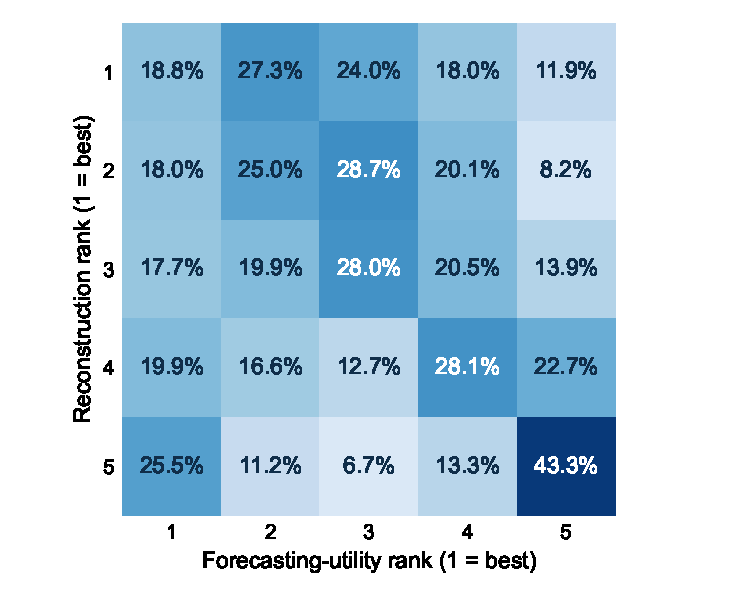
\includegraphics[width=0.75\textwidth]{figure/fig6_rank_agreement.eps}
  \caption{Within-episode reconstruction rank against forecasting-utility rank for the five repairs. Each row is normalised to $100\%$ up to rounding. Concentration away from the diagonal shows disagreement between the criteria. Cells reproduce the recorded table percentages.}
  \label{fig:rankgrid}
\end{figure}

\begin{table}[htbp]
  \caption{Reconstruction quality against realised forecasting utility, over the five catalog
  interventions on the reused evaluation episodes of the Bolt backbone. Reconstruction error is measured on the
  hidden positions and realised utility against \textsc{Keep} on the same backbone. Winner
  agreement is the share of episodes on which the most accurate reconstruction is also the most
  useful intervention, and the discordant rate is the share of ordered pairs whose two rankings
  disagree.}
  \label{tab:app-recutils}
  \centering
  \small
  \setlength{\tabcolsep}{4pt}
\adjustbox{max width=\textwidth}{\begin{tabular}{lcccc}
    \toprule
    Intervention & Rec.\ MSE $\downarrow$ & Rec.\ MAE $\downarrow$
                 & Mean realised utility $\uparrow$ & Episodes \\
    \midrule
    \textsc{Ffill}         & 77.47  & 4.08  & -0.139  & 760 \\
    \textsc{Single TS-ICL} & 29.61 & 2.03 & +0.013 & 760 \\
    \textsc{Multi TS-ICL}  & 29.59  & 1.85  & +0.029  & 758 \\
    \textsc{Context Ridge} & 30.39  & 1.48  & +0.043  & 566 \\
    \textsc{SAITS}         & 68.25  & 3.10  & +0.037  & 747 \\
    \midrule
    \multicolumn{5}{l}{\footnotesize Winner agreement 19.3\%, discordant rate
    44.5\%, mean within-episode Spearman $\rho$ 0.12} \\
    \bottomrule
  \end{tabular}}
\end{table}

Reconstruction and forecasting utility favour different actions in these diagnostics.
The weak rank agreement motivates direct evaluation of forecasting utility when selecting
repairs. It does not establish that reconstruction quality is uninformative in every setting.

\subsection{Where an Action's Utility Comes From}
\label{app:utility-by-severity}
Table~\ref{tab:app-utility-severity} reports the mean realised utility of each catalog action
on the replay bank, once over the whole bank and once within each registered severity. It
selects nothing and is computed after the configuration was frozen. Two things in it matter for
reading the main tables.

The recorded action utilities vary with both backbone and severity. Several repairs become
more useful as missingness increases on TimesFM, while the Chronos-2 values change less.
This variation motivates reporting each backbone separately and assessing severity sensitivity.

For Bolt, the recorded mean utility of \textsc{Context Ridge} is $+0.073$ across the bank
and $+0.036$ at $10\%$ missingness. These summaries use different severity mixtures.
Their difference alone does not identify an outlier or establish its causal contribution.
Raw outcomes must be retained when examining the effect of extreme repairs.

\begin{table}[htbp]
  \caption{Mean realised utility of each action on the replay bank, overall and within each
  registered severity. Positive means the action lowered the forecasting loss relative to
  leaving the input unchanged. Utility is measured per episode, so it is not on the same
  aggregation as the source-macro MASE of the main tables and the two are not directly
  comparable in magnitude.}
  \label{tab:app-utility-severity}
  \centering
  \small
  \setlength{\tabcolsep}{4pt}
\adjustbox{max width=\textwidth}{\begin{tabular}{llcccc}
    \toprule
    Backbone & Action & All severities & $10\%$ & $30\%$ & $50\%$ \\
    \midrule
    \multirow{4}{*}{Bolt}
      & \textsc{Ffill}         & -0.167  & -0.130  & -0.162  & -0.209 \\
      & \textsc{Single TS-ICL} & +0.018 & +0.002 & +0.006 & +0.045 \\
      & \textsc{Multi TS-ICL}  & +0.035  & +0.013  & +0.036  & +0.057 \\
      & \textsc{Context Ridge} & +0.073  & +0.036  & +0.052  & +0.136 \\
    \midrule
    \multirow{4}{*}{TimesFM}
      & \textsc{Ffill}         & -0.022  & -0.013  & -0.025  & -0.029 \\
      & \textsc{Single TS-ICL} & +0.191 & +0.131 & +0.187 & +0.254 \\
      & \textsc{Multi TS-ICL}  & +0.205  & +0.145  & +0.210  & +0.261 \\
      & \textsc{Context Ridge} & +0.310  & +0.216  & +0.304  & +0.419 \\
    \midrule
    \multirow{4}{*}{Chronos-2}
      & \textsc{Ffill}         & -0.180  & -0.120  & -0.177  & -0.242 \\
      & \textsc{Single TS-ICL} & -0.002 & -0.007 & -0.001 & +0.002 \\
      & \textsc{Multi TS-ICL}  & +0.026  & +0.012  & +0.038  & +0.029 \\
      & \textsc{Context Ridge} & +0.096  & +0.068  & +0.095  & +0.128 \\
    \bottomrule
  \end{tabular}}
\end{table}

\subsection{Per-Source Results}
\label{app:datasets}
Each table below reports one frozen backbone at $10\%$ severity, one horizon, and
all eight sources, with one row per method. MASE is reported in every cell so that a
reader can recompute the source-macro aggregate of Table~\ref{tab:main} directly from
these tables. The \emph{macro} column is the equal-weight average over the eight sources
and is the quantity the main table reports. Rows are generated from the recorded result
group using the same aggregation as the main table.
MAE and RMSE are reported per source and are not averaged across sources.

\begin{table}[htbp]
  \caption{Per-source MASE on Bolt at $10\%$ severity, $H=96$. The macro column is the
  equal-weight average over the eight sources and is the quantity reported in
  Table~\ref{tab:main}. Lower is better everywhere.}
  \label{tab:app-src-bolt-96}
  \centering
  \small
  \setlength{\tabcolsep}{3pt}
\adjustbox{max width=\textwidth}{\begin{tabular}{lcccccccc c}
    \toprule
    Method & ETTh1 & ETTh2 & ETTm1 & ETTm2 & Electricity & Exchange & Traffic & Weather & Macro $\downarrow$ \\
    \midrule
    Native KEEP & 0.967 & 1.444 & 1.370 & 1.035 & 0.957 & 2.761 & 0.980 & 0.645 & 1.270 \\
    Best Fixed & 0.877 & 1.293 & 1.321 & 1.015 & 0.951 & 2.784 & 0.955 & 0.651 & 1.231 \\
    R2-CART & 0.886 & 1.319 & 1.312 & 1.002 & 0.911 & 2.535 & 0.908 & 0.633 & 1.188 \\
    Fixed SAITS & 0.878 & 1.280 & 1.306 & 0.993 & 0.998 & 3.418 & 0.887 & 0.638 & 1.300 \\
    TATO & 1.421 & 1.364 & 1.713 & 1.120 & 0.892 & 2.385 & 1.485 & 0.672 & 1.382 \\
    \midrule
    \rowcolor{bestgray}\introact{} & 0.881 & 1.283 & 1.318 & 1.009 & 0.921 & 2.404 & 0.917 & 0.653 & 1.173 \\
    \midrule
    Catalog Oracle & \oracle{0.830} & \oracle{1.170} & \oracle{1.196} & \oracle{0.926} & \oracle{0.712} & \oracle{2.288} & \oracle{0.836} & \oracle{0.454} & \oracle{1.052} \\
    \bottomrule
  \end{tabular}}
\end{table}

\begin{table}[htbp]
  \caption{Per-source MASE on Bolt at $10\%$ severity, $H=192$. The macro column is the
  equal-weight average over the eight sources and is the quantity reported in
  Table~\ref{tab:main}. Lower is better everywhere.}
  \label{tab:app-src-bolt-192}
  \centering
  \small
  \setlength{\tabcolsep}{3pt}
\adjustbox{max width=\textwidth}{\begin{tabular}{lcccccccc c}
    \toprule
    Method & ETTh1 & ETTh2 & ETTm1 & ETTm2 & Electricity & Exchange & Traffic & Weather & Macro $\downarrow$ \\
    \midrule
    Native KEEP & 1.082 & 1.447 & 1.415 & 1.239 & 0.870 & 5.071 & 1.018 & 1.162 & 1.663 \\
    Best Fixed & 1.031 & 1.348 & 1.385 & 1.217 & 0.878 & 5.019 & 0.997 & 1.125 & 1.625 \\
    R2-CART & 1.037 & 1.352 & 1.389 & 1.215 & 0.895 & 4.910 & 0.986 & 1.145 & 1.616 \\
    Fixed SAITS & 1.025 & 1.333 & 1.384 & 1.187 & 0.968 & 5.165 & 0.971 & 1.075 & 1.638 \\
    TATO & 1.510 & 1.528 & 1.682 & 1.310 & 0.898 & 5.074 & 1.590 & 1.278 & 1.859 \\
    \midrule
    \rowcolor{bestgray}\introact{} & 1.031 & 1.341 & 1.378 & 1.208 & 0.906 & 4.690 & 0.983 & 1.131 & 1.583 \\
    \midrule
    Catalog Oracle & \oracle{0.994} & \oracle{1.248} & \oracle{1.286} & \oracle{1.130} & \oracle{0.685} & \oracle{4.191} & \oracle{0.920} & \oracle{0.882} & \oracle{1.417} \\
    \bottomrule
  \end{tabular}}
\end{table}

\begin{table}[htbp]
  \caption{Per-source MASE on TimesFM at $10\%$ severity, $H=96$. The macro column is the
  equal-weight average over the eight sources and is the quantity reported in
  Table~\ref{tab:main}. Lower is better everywhere.}
  \label{tab:app-src-tf-96}
  \centering
  \small
  \setlength{\tabcolsep}{3pt}
\adjustbox{max width=\textwidth}{\begin{tabular}{lcccccccc c}
    \toprule
    Method & ETTh1 & ETTh2 & ETTm1 & ETTm2 & Electricity & Exchange & Traffic & Weather & Macro $\downarrow$ \\
    \midrule
    Native KEEP & 1.235 & 1.363 & 1.568 & 1.155 & 0.963 & 3.330 & 1.199 & 0.628 & 1.430 \\
    Best Fixed & 0.979 & 1.229 & 1.133 & 1.017 & 0.831 & 3.607 & 0.908 & 0.661 & 1.296 \\
    R2-CART & 0.998 & 1.264 & 1.149 & 1.002 & 0.885 & 3.579 & 0.901 & 0.621 & 1.300 \\
    Fixed SAITS & 0.970 & 1.244 & 1.117 & 0.992 & 0.870 & 2.996 & 0.906 & 0.629 & 1.216 \\
    TATO & 1.359 & 1.226 & 1.692 & 1.175 & 1.102 & 2.740 & 1.249 & 0.710 & 1.407 \\
    \midrule
    \rowcolor{bestgray}\introact{} & 1.012 & 1.218 & 1.142 & 1.008 & 0.934 & 3.187 & 0.908 & 0.630 & 1.255 \\
    \midrule
    Catalog Oracle & \oracle{0.896} & \oracle{1.144} & \oracle{1.041} & \oracle{0.944} & \oracle{0.633} & \oracle{2.568} & \oracle{0.860} & \oracle{0.463} & \oracle{1.069} \\
    \bottomrule
  \end{tabular}}
\end{table}

\begin{table}[htbp]
  \caption{Per-source MASE on TimesFM at $10\%$ severity, $H=192$. The macro column is the
  equal-weight average over the eight sources and is the quantity reported in
  Table~\ref{tab:main}. Lower is better everywhere.}
  \label{tab:app-src-tf-192}
  \centering
  \small
  \setlength{\tabcolsep}{3pt}
\adjustbox{max width=\textwidth}{\begin{tabular}{lcccccccc c}
    \toprule
    Method & ETTh1 & ETTh2 & ETTm1 & ETTm2 & Electricity & Exchange & Traffic & Weather & Macro $\downarrow$ \\
    \midrule
    Native KEEP & 1.232 & 1.391 & 1.688 & 1.332 & 1.021 & 6.475 & 1.197 & 1.135 & 1.934 \\
    Best Fixed & 1.110 & 1.304 & 1.294 & 1.217 & 0.905 & 6.914 & 0.996 & 1.152 & 1.862 \\
    R2-CART & 1.106 & 1.334 & 1.299 & 1.206 & 0.898 & 7.044 & 1.007 & 1.123 & 1.877 \\
    Fixed SAITS & 1.098 & 1.327 & 1.285 & 1.193 & 0.926 & 5.769 & 0.990 & 1.133 & 1.715 \\
    TATO & 1.367 & 1.303 & 1.784 & 1.342 & 1.228 & 5.063 & 1.273 & 1.208 & 1.821 \\
    \midrule
    \rowcolor{bestgray}\introact{} & 1.132 & 1.268 & 1.295 & 1.214 & 0.976 & 6.803 & 0.995 & 1.137 & 1.853 \\
    \midrule
    Catalog Oracle & \oracle{1.040} & \oracle{1.198} & \oracle{1.229} & \oracle{1.122} & \oracle{0.761} & \oracle{5.304} & \oracle{0.960} & \oracle{0.883} & \oracle{1.562} \\
    \bottomrule
  \end{tabular}}
\end{table}

\begin{table}[htbp]
  \caption{Per-source MASE on Chronos-2 at $10\%$ severity, $H=96$. The macro column is the
  equal-weight average over the eight sources and is the quantity reported in
  Table~\ref{tab:main}. Lower is better everywhere.}
  \label{tab:app-src-ch2-96}
  \centering
  \small
  \setlength{\tabcolsep}{3pt}
\adjustbox{max width=\textwidth}{\begin{tabular}{lcccccccc c}
    \toprule
    Method & ETTh1 & ETTh2 & ETTm1 & ETTm2 & Electricity & Exchange & Traffic & Weather & Macro $\downarrow$ \\
    \midrule
    Native KEEP & 1.083 & 1.238 & 1.288 & 1.016 & 0.768 & 3.272 & 0.857 & 0.668 & 1.274 \\
    Best Fixed & 1.020 & 1.120 & 1.192 & 1.007 & 0.795 & 2.781 & 0.836 & 0.651 & 1.175 \\
    R2-CART & 1.016 & 1.114 & 1.195 & 1.003 & 0.773 & 2.380 & 0.836 & 0.637 & 1.119 \\
    Fixed SAITS & 1.021 & 1.134 & 1.191 & 0.977 & 0.852 & 2.722 & 0.825 & 0.634 & 1.170 \\
    TATO & 1.438 & 1.649 & 1.617 & 1.183 & 1.028 & 2.641 & 1.284 & 0.650 & 1.436 \\
    \midrule
    \rowcolor{bestgray}\introact{} & 1.019 & 1.210 & 1.221 & 0.985 & 0.833 & 2.152 & 0.822 & 0.643 & 1.111 \\
    \midrule
    Catalog Oracle & \oracle{0.936} & \oracle{1.017} & \oracle{1.082} & \oracle{0.921} & \oracle{0.590} & \oracle{1.992} & \oracle{0.790} & \oracle{0.461} & \oracle{0.974} \\
    \bottomrule
  \end{tabular}}
\end{table}

\begin{table}[htbp]
  \caption{Per-source MASE on Chronos-2 at $10\%$ severity, $H=192$. The macro column is the
  equal-weight average over the eight sources and is the quantity reported in
  Table~\ref{tab:main}. Lower is better everywhere.}
  \label{tab:app-src-ch2-192}
  \centering
  \small
  \setlength{\tabcolsep}{3pt}
\adjustbox{max width=\textwidth}{\begin{tabular}{lcccccccc c}
    \toprule
    Method & ETTh1 & ETTh2 & ETTm1 & ETTm2 & Electricity & Exchange & Traffic & Weather & Macro $\downarrow$ \\
    \midrule
    Native KEEP & 1.175 & 1.298 & 1.362 & 1.221 & 0.842 & 6.940 & 0.966 & 1.275 & 1.885 \\
    Best Fixed & 1.133 & 1.323 & 1.299 & 1.233 & 0.857 & 5.862 & 0.956 & 1.238 & 1.738 \\
    R2-CART & 1.131 & 1.345 & 1.298 & 1.229 & 0.857 & 5.195 & 0.944 & 1.200 & 1.650 \\
    Fixed SAITS & 1.116 & 1.286 & 1.305 & 1.200 & 0.936 & 5.748 & 0.949 & 1.161 & 1.713 \\
    TATO & 1.457 & 1.908 & 1.656 & 1.349 & 1.086 & 4.493 & 1.253 & 1.138 & 1.792 \\
    \midrule
    \rowcolor{bestgray}\introact{} & 1.150 & 1.312 & 1.309 & 1.189 & 0.887 & 5.132 & 0.954 & 1.230 & 1.645 \\
    \midrule
    Catalog Oracle & \oracle{1.048} & \oracle{1.152} & \oracle{1.210} & \oracle{1.107} & \oracle{0.699} & \oracle{4.744} & \oracle{0.915} & \oracle{0.948} & \oracle{1.478} \\
    \bottomrule
  \end{tabular}}
\end{table}

\subsection{Per-Pattern Results}
\label{app:pattern}
Table~\ref{tab:app-pattern-res} separates the four patterns. Point missing is expected to
be the easiest regime and tail missing the hardest, because the missing block is adjacent
to the forecast origin and therefore removes exactly the observations a forecaster would
rely on most. Any claim about a pattern is a claim about this table, not about the pooled
main table.

\begin{table}[htbp]
  \caption{Per-pattern MASE at $10\%$ severity, source-macro averaged over the three
  backbones and both horizons. The last column ranks the deployable methods per request
  within each pattern and macro-averages those ranks over the four patterns; because every
  pattern holds the same number of requests, this equals the per-request average rank of
  Table~\ref{tab:main}.}
  \label{tab:app-pattern-res}
  \centering
  \small
  \setlength{\tabcolsep}{4pt}
\adjustbox{max width=\textwidth}{\begin{tabular}{lccccc}
    \toprule
    Method & P1 Point & P2 Target Block & P3 Shared Block & P4 Tail & Avg.\ Rank $\downarrow$ \\
    \midrule
    \textsc{Native Keep} & 1.436 & 1.379 & 1.400 & 2.088 & 3.36 \\
    \textsc{Best Fixed}  & 1.412   & 1.393   & 1.400   & 1.746   & 2.94 \\
    R2-CART              & 1.409   & 1.439   & 1.425   & 1.561   & 2.97 \\
    Fixed SAITS & 1.318 & 1.425 & 1.549 & 1.543 & 2.98 \\
    TATO & 1.336 & 1.371 & 1.317 & 2.441 & 4.10 \\
    \midrule
    \rowcolor{bestgray}\introact{} & 1.376 & 1.381 & 1.386 & 1.604 & 2.79 \\
    \bottomrule
  \end{tabular}}
\end{table}

\subsection{Source-Level Fixed Policy and Leave-One-Source-Out}
\label{app:source-diagnostics}
This subsection supports the source-attribution question of \S\ref{sec:exp-main}. The
checks were run on the retained prediction cache with selection confined to the TRAIN
side, and all TEST numbers remain post-hoc comparisons on the previously examined block.
Intervals are the recorded 2,000-resample paired parent-bootstrap intervals (seed 101),
nominal and without multiple-comparison adjustment.

The source-level fixed policy applies, per source, the single catalog action with the
highest mean realised utility on the replay bank, with \textsc{Keep} as the registered
fallback where that action is unsupported (fallback counts are recorded with the result;
the largest is 48 of 190 requests on ETTm1 and ETTm2, whose chosen action is Context
Ridge). The chosen action varies by source and backbone — Context Ridge dominates (16 of
the 24 source-backbone pairs), with Multi TS-ICL, Single TS-ICL, FFILL and SAITS each
selected somewhere — so the policy tests whether
source identity alone carries the gain.

\begin{table}[htbp]
\centering\small
\caption{Source-level fixed policy on TEST against the full rule. The difference is FULL
minus the source-level fixed policy, so a positive value favours the fixed policy.}
\label{tab:v53-source-fixed}
\begin{tabular}{lcccl}
\toprule
Backbone & FULL MASE & Source-fixed MASE & Intervention rate & FULL$-$fixed [interval] \\
\midrule
Bolt & 1.3783 & 1.3602 & 82.6\% & $+0.0181$ [$0.0061$, $0.0296$] \\
TimesFM & 1.5537 & 1.5268 & 80.3\% & $+0.0269$ [$0.0035$, $0.0526$] \\
Chronos-2 & 1.3779 & 1.4484 & 83.4\% & $-0.0704$ [$-0.1558$, $0.0156$] \\
\bottomrule
\end{tabular}
\end{table}

\begin{table}[htbp]
\centering\small
\caption{Leave-one-source-out on TEST: the FULL-minus-control difference in source-macro
MASE with each source removed in turn. Only the full set and the Exchange-excluded subset
are printed; the remaining seven rows per backbone move monotonically between these two
and are recorded with the result files. A negative value favours FULL.}
\label{tab:v53-loso}
\adjustbox{max width=\textwidth}{\begin{tabular}{llccccc}
\toprule
Backbone & Subset & vs KEEP & vs Best Fixed & vs R2-CART & vs Fixed SAITS & vs TATO \\
\midrule
Bolt & all eight & $-0.0881$ & $-0.0497$ & $-0.0239$ & $-0.0908$ & $-0.2418$ \\
Bolt & without Exchange & $-0.0480$ & $-0.0061$ & $-0.0023$ & $+0.0025$ & $-0.2503$ \\
TimesFM & all eight & $-0.1283$ & $-0.0249$ & $-0.0348$ & $+0.0884$ & $-0.0602$ \\
TimesFM & without Exchange & $-0.1599$ & $+0.0095$ & $+0.0055$ & $+0.0135$ & $-0.2250$ \\
Chronos-2 & all eight & $-0.2014$ & $-0.0785$ & $-0.0067$ & $-0.0631$ & $-0.2365$ \\
Chronos-2 & without Exchange & $-0.0211$ & $+0.0073$ & $+0.0131$ & $+0.0125$ & $-0.2810$ \\
\bottomrule
\end{tabular}}
\end{table}

The margin over the unchanged input keeps its sign on all eight subsets of every backbone,
although on Chronos-2 it too is concentrated in Exchange. The margins over Best Fixed and
R2-CART vanish or reverse without Exchange on all three backbones. Together with
Table~\ref{tab:v53-source-fixed}, this bounds the claim the evaluation supports: selective
repair improves on leaving the input unchanged across sources, but its advantage over the
stronger simple controls is carried substantially by one source, and on two backbones a
per-source fixed choice is at least as accurate as per-request selection.

\section{Intervention Frequency and Harm}

This section supports \S\ref{sec:exp-harm}; it collects the default operating point, the
action-opportunity strata, and the complete tables of every frequency comparison.

\subsection{Governance Diagnostics}
\label{app:governance-fig}
Table~\ref{tab:app-operating} reports operating points across the penalty grid and
Table~\ref{tab:app-scorebins} checks that the order the score induces agrees with the sign of
the realised utility. The score is used only to order actions, and its magnitude is not claimed
to be calibrated against the utility scale. Over 10773 admissible pairs the sign of the score and the sign of the realised utility agree on 54\% of them, and the mean realised utility is +0.197 where the score is positive against -0.031 where it is negative, so the score provides limited directional evidence without calibrated utility estimates.

\begin{table}[htbp]
  \caption{Operating points over the penalty grid, with the neighbourhood size frozen at the
  selected value on each backbone. Intervention rate is the share of requests on which a
  non-reference action ran, and conditional HIR is the share of those that raised the loss.
  Raising the penalty moves the rate and leaves the conditional rate close to where it was, so
  the largest change is in intervention frequency.}
  \label{tab:app-operating}
  \centering
  \small
  \setlength{\tabcolsep}{4pt}
\adjustbox{max width=\textwidth}{\begin{tabular}{lcccccc}
    \toprule
     & \multicolumn{2}{c}{Bolt} & \multicolumn{2}{c}{TimesFM} & \multicolumn{2}{c}{Chronos-2} \\
    \cmidrule(lr){2-3}\cmidrule(lr){4-5}\cmidrule(lr){6-7}
    Penalty strength & Int.\ rate & Cond.\ HIR & Int.\ rate & Cond.\ HIR & Int.\ rate & Cond.\ HIR \\
    \midrule
    $\beta = 0$ & 87.2\% & 42.2\% & 92.2\% & 42.7\% & 78.9\% & 40.2\% \\
    $\beta = 0.5$ & 74.6\% & 42.2\% & 84.7\% & 40.7\% & 69.1\% & 39.6\% \\
    $\beta = 1$ & 64.6\% & 43.0\% & 69.3\% & 41.4\% & 54.6\% & 37.3\% \\
    $\beta = 1.64$ & 48.2\% & 42.9\% & 52.4\% & 38.7\% & 36.6\% & 41.0\% \\
    \bottomrule
  \end{tabular}}
\end{table}

\begin{table}[htbp]
  \caption{Realised utility against the quantile bin of the conservative score, pooled over the
  three backbones and every admissible action. The score orders actions and its magnitude is
  not claimed to be calibrated, so what this table checks is whether the order it induces
  agrees with the sign of the utility. Intervals resample parents.}
  \label{tab:app-scorebins}
  \centering
  \small
  \setlength{\tabcolsep}{4pt}
\begin{tabular}{lccc}
    \toprule
    Score bin & Pairs & Mean realised utility & 95\% interval \\
    \midrule
    1 (lowest score) & 2,157 & -0.105 & [-0.250, +0.047] \\
    2 & 2,154 & +0.007 & [-0.009, +0.032] \\
    3 & 2,154 & +0.008 & [-0.033, +0.035] \\
    4 & 2,154 & +0.017 & [-0.007, +0.052] \\
    5 (highest score) & 2,154 & +0.304 & [+0.058, +0.788] \\
    \bottomrule
  \end{tabular}
\end{table}

\subsection{Action-Opportunity Strata}
\label{app:opportunity}
This subsection supports \S\ref{sec:exp-exists}. For an evaluation episode $i$ the oracle
opportunity is the improvement the best admissible action could have produced over the
reference input,
\begin{equation}
  \Delta_i \;=\; \loss\!\left(F(T_{a_0}(X_i, M_i)),\, y_i\right) - \min_{a \in \calA} \loss\!\left(F(T_{a}(X_i, M_i)),\, y_i\right),
  \label{eq:opportunity}
\end{equation}
which uses the realised target and is therefore a retrospective diagnostic. Episodes are partitioned into a \emph{no-op} stratum, where the reference input is
already best up to a tolerance, a \emph{low-opportunity} stratum, and a
\emph{high-opportunity} stratum. The two boundaries are fitted on the replay bank and applied
unchanged to TEST, so no evaluation episode participates in choosing them.
Table~\ref{tab:app-opp-sizes} records the realised stratum sizes,
Table~\ref{tab:app-opportunity} reports source-macro MASE within each stratum under the
identical partition for every method, and Table~\ref{tab:app-opp-sens} repeats the
stratum-level MASE under alternative boundaries so that a reader can see how much of the
effect depends on where the boundary was drawn.

\begin{table}[htbp]
  \caption{Action-opportunity strata on TEST. Boundaries are the bank thresholds, applied
  unchanged. Counts are of parents and not of mask variants.}
  \label{tab:app-opp-sizes}
  \centering
  \small
  \setlength{\tabcolsep}{4pt}
\adjustbox{max width=\textwidth}{\begin{tabular}{lcccc}
    \toprule
    Stratum & Parents & Share of episodes & Median $\Delta_i$ & 90th pct.\ $\Delta_i$ \\
    \midrule
    No-op             & 68  & 19.3\%  & 0.000  & 0.000 \\
    Low opportunity   & 91   & 47.1\%   & 0.038   & 0.100 \\
    High opportunity  & 79  & 33.5\%  & 0.352  & 1.293 \\
    \bottomrule
  \end{tabular}}
\end{table}

\begin{table}[htbp]
  \caption{Stratum-level MASE under the identical partition. The no-op stratum is where an
  intervention can only lose, so a method that is better only in the high-opportunity stratum
  while degrading the no-op stratum has not solved the selection problem. Lower is better.}
  \label{tab:app-opportunity}
  \centering
  \small
  \setlength{\tabcolsep}{4pt}
\adjustbox{max width=\textwidth}{\begin{tabular}{lcccc}
    \toprule
    Method & No-op MASE $\downarrow$ & Low opportunity $\downarrow$ & High opportunity $\downarrow$ & Overall $\downarrow$ \\
    \midrule
    Native KEEP        & 1.287    & 1.166    & 2.039    & 1.576 \\
    Best Fixed         & 1.401      & 1.181      & 1.689      & 1.488 \\
    R2-CART            & 1.490      & 1.197      & 1.588      & 1.458 \\
    Fixed SAITS           & 1.565      & 1.225      & 1.554      & 1.459 \\
    TATO               & 1.444    & 1.245    & 2.177    & 1.616 \\
    \midrule
    \rowcolor{bestgray}\introact{} & 1.389 & 1.170 & 1.652 & 1.437 \\
    \bottomrule
  \end{tabular}}
\end{table}

\begin{table}[htbp]
  \caption{Stratum-boundary sensitivity. The no-op tolerance and the low and high boundary are
  shifted by the indicated factor of the bank threshold, and every other setting is unchanged.
  MASE is source-macro averaged within the resulting strata.}
  \label{tab:app-opp-sens}
  \centering
  \small
  \setlength{\tabcolsep}{4pt}
\adjustbox{max width=\textwidth}{\begin{tabular}{lcccc}
    \toprule
    Boundary factor & No-op MASE $\downarrow$ & Low MASE $\downarrow$ & High MASE $\downarrow$ & Overall MASE $\downarrow$ \\
    \midrule
    $\times 0.5$ & 1.389  & 1.056  & 1.513  & 1.437 \\
    $\times 1.0$ & 1.389   & 1.170   & 1.652   & 1.437 \\
    $\times 2.0$ & 1.389   & 1.433   & 2.707   & 1.437 \\
    \bottomrule
  \end{tabular}}
\end{table}

\subsection{Gate Controls}
\label{app:gate-controls}
Table~\ref{tab:v52-gates} compares the frozen gate against post-hoc controls on TEST.
These controls were run after reviewing the earlier TEST results; they use the retained
prediction cache and the frozen full-method settings, and they do not constitute an
independent confirmation set. All intervals in this subsection are the recorded
10,000-resample paired parent-bootstrap intervals and are nominal, without
multiple-comparison adjustment.

\begin{table}[htbp]
\centering\small
\caption{Gate controls on TEST. Thresholds and random acceptance probabilities were
calibrated on the development block. HIR is conditional on an intervention.}
\label{tab:v52-gates}
\begin{tabular}{llrrrr}
\toprule
Backbone & Rule & MASE & Intervention (\%) & HIR (\%) & Harmful loss \\
\midrule
Bolt & FULL & 1.3783 & 74.61 & 42.15 & 0.03769 \\
Bolt & Mean only & 1.3765 & 75.66 & 42.61 & 0.03986 \\
Bolt & Linear & 1.4046 & 71.32 & 43.36 & 0.04685 \\
Bolt & Random & 1.4075 & 75.13 & 41.86 & 0.03545 \\
TimesFM & FULL & 1.5537 & 52.37 & 38.69 & 0.03701 \\
TimesFM & Mean only & 1.6078 & 52.11 & 39.65 & 0.05270 \\
TimesFM & Linear & 1.5389 & 51.45 & 36.83 & 0.04335 \\
TimesFM & Random & 1.6719 & 47.37 & 43.61 & 0.02913 \\
Chronos-2 & FULL & 1.3779 & 69.08 & 39.62 & 0.03786 \\
Chronos-2 & Mean only & 1.3753 & 68.82 & 40.73 & 0.03912 \\
Chronos-2 & Linear & 1.3706 & 69.61 & 44.42 & 0.04653 \\
Chronos-2 & Random & 1.4462 & 71.58 & 41.54 & 0.03504 \\
\bottomrule
\end{tabular}
\end{table}

The random control uses a single recorded seed, 101. Its intervals resample parents and
do not include variability over random-gate seeds. The mean-only and linear controls change
both recommendations and acceptance scores, so their comparisons do not isolate the penalty
alone. No TEST outcome is used to rematch their realised intervention frequencies.

\subsection{Frequency-Matched Comparison Partners}
\label{app:matched-partners}
These checks were run on the same retained prediction cache as the gate controls.
Intervals are the recorded 2,000-resample paired parent-bootstrap intervals (seed 101),
nominal and without multiple-comparison adjustment.

Table~\ref{tab:v53-gates} extends the gate controls of Appendix~\ref{app:gate-controls} from generic
gates to the comparison partners themselves. R2-CART-M recalibrates the simple selector's
acceptance threshold on the development block to the full method's development intervention
rate (thresholds $0.590$, $0.658$, $0.617$ per backbone); the tree's discrete probabilities
and tied quantiles make the realised TEST rates lower than the targets, most visibly on
Chronos-2, and no rematching is done. BF-Random executes the best fixed repair with a
per-request hash probability calibrated the same way; its realised TEST rates are further
reduced by the fixed repair's unsupported requests. Both are frozen before TEST is read.

\begin{table}[htbp]
\centering\small
\caption{Frequency-matched comparison partners on TEST. Differences are FULL minus the
named control; a negative value favours FULL. HIR is conditional on an intervention.}
\label{tab:v53-gates}
\adjustbox{max width=\textwidth}{\begin{tabular}{llrrrrl}
\toprule
Backbone & Control & MASE & Intervention (\%) & HIR (\%) & Harmful loss & FULL$-$control [interval] \\
\midrule
Bolt & R2-CART, default threshold & 1.4022 & 100.0 & 43.7 & 0.0478 & $-0.0239$ [$-0.0490$, $0.0009$] \\
Bolt & R2-CART-M, matched & 1.4035 & 72.8 & 41.2 & 0.0358 & $-0.0252$ [$-0.0495$, $-0.0011$] \\
Bolt & BF-Random, matched & 1.4423 & 52.2 & 42.3 & 0.0337 & $-0.0640$ [$-0.1167$, $-0.0114$] \\
TimesFM & R2-CART, default threshold & 1.5885 & 99.2 & 41.4 & 0.0666 & $-0.0348$ [$-0.0921$, $0.0221$] \\
TimesFM & R2-CART-M, matched & 1.5899 & 42.9 & 35.3 & 0.0323 & $-0.0362$ [$-0.0940$, $0.0222$] \\
TimesFM & BF-Random, matched & 1.6389 & 33.7 & 40.2 & 0.0291 & $-0.0852$ [$-0.1338$, $-0.0371$] \\
Chronos-2 & R2-CART, default threshold & 1.3846 & 98.9 & 44.1 & 0.0609 & $-0.0067$ [$-0.0437$, $0.0316$] \\
Chronos-2 & R2-CART-M, matched & 1.4121 & 46.1 & 41.1 & 0.0296 & $-0.0342$ [$-0.0745$, $0.0062$] \\
Chronos-2 & BF-Random, matched & 1.4963 & 49.6 & 43.0 & 0.0315 & $-0.1183$ [$-0.1927$, $-0.0438$] \\
\bottomrule
\end{tabular}}
\end{table}

The full rule separates from the frequency-matched random fixed policy on every backbone,
which frequency reduction alone cannot explain. It separates from the frequency-matched
simple selector only on Bolt, so the advantage over R2-CART is not established as a
frequency-independent effect on the other two backbones. Harmful loss of both matched
controls is lower than the full rule's on every backbone: the full rule spends its
interventions more accurately, not more safely.

\section{Estimation and State Analyses}

This section supports \S\ref{sec:exp-ablation} and separates the fixed-configuration
ablations from the representation comparisons that re-run selection.

\subsection{Ablation Details}
\label{app:ablation-details}
This section supports \S\ref{sec:exp-ablation}. Every variant reads the same catalog
prediction cache, so the rows differ only in how the stored utilities are summarised and
thresholded. Table~\ref{tab:app-ablation} reports the full outcome vector behind the compact
Table~\ref{tab:ablation}. The variant definitions follow \S\ref{sec:exp-ablation} exactly.

\begin{table}[htbp]
  \caption{Ablation, full outcome vector in the two scaled metrics. Raw errors are not
  averaged across sources anywhere in this paper, so they are not shown here either. Calls
  counts forecasting-backbone calls per request and harmful loss is relative to
  \textsc{Keep}.}
  \label{tab:app-ablation}
  \centering
  \small
  \setlength{\tabcolsep}{4pt}
\adjustbox{max width=\textwidth}{\begin{tabular}{lcccccc}
    \toprule
    Variant & MASE $\downarrow$ & RMSSE $\downarrow$ & Intervention rate & Conditional HIR $\downarrow$ & Harmful loss $\downarrow$ & Calls $\downarrow$ \\
    \midrule
    Full \introact{}            & 1.437 & 1.233 & 65.4\% & 40.2\% & 0.0375 & 1.65 \\
    A1 Global utility & 1.475 & 1.255 & 100.0\% & 43.9\% & 0.0697 & 2.00 \\
    A2 w/o intervention state & 1.418 & 1.219 & 63.4\% & 39.5\% & 0.0330 & 1.63 \\
    A3 w/o reference-forecast state & 1.446 & 1.240 & 67.4\% & 40.4\% & 0.0419 & 1.67 \\
    A4 Always act & 1.447 & 1.239 & 100.0\% & 42.1\% & 0.0533 & 2.00 \\
    A5 Parametric utility predictor & 1.434 & 1.234 & 86.7\% & 43.7\% & 0.0549 & 1.87 \\
    \midrule
    \bottomrule
  \end{tabular}}
\end{table}

\subsection{Mechanism and Feature Controls}
\label{app:estimation-analyses}
These controls were run after reviewing the earlier TEST results; they use the retained
prediction cache and the frozen full-method settings, and they do not constitute an
independent confirmation set. All intervals in this subsection are the recorded
10,000-resample paired parent-bootstrap intervals and are nominal, without
multiple-comparison adjustment.

A2-M pools neighbours across all repair actions, with global action-wise
utility priors. A2-F removes the five intervention features while
retaining same-action retrieval. These answer different questions. Neither result justifies
relabeling A2-F as a mechanism ablation or suppressing its favourable error.

\begin{table}[htbp]
\centering\small
\caption{Distinct mechanism and feature controls. Differences are FULL minus the named
control. Negative values favour FULL.}
\label{tab:v52-a2}
\begin{tabular}{llrrl}
\toprule
Backbone & Control & MASE & Difference & Nominal 95\% interval \\
\midrule
Bolt & Pooled utilities & 1.4035 & -0.0252 & $[-0.0478,-0.0025]$ \\
Bolt & Omit intervention features & 1.3623 & +0.0160 & $[0.0025,0.0293]$ \\
Bolt & Linear utility & 1.3969 & -0.0185 & $[-0.0445,0.0072]$ \\
TimesFM & Pooled utilities & 1.5555 & -0.0018 & $[-0.0335,0.0310]$ \\
TimesFM & Omit intervention features & 1.5179 & +0.0358 & $[-0.0049,0.0772]$ \\
TimesFM & Linear utility & 1.5417 & +0.0120 & $[-0.0076,0.0315]$ \\
Chronos-2 & Pooled utilities & 1.3819 & -0.0040 & $[-0.0337,0.0265]$ \\
Chronos-2 & Omit intervention features & 1.3752 & +0.0027 & $[-0.0014,0.0071]$ \\
Chronos-2 & Linear utility & 1.3644 & +0.0136 & $[-0.0126,0.0398]$ \\
\bottomrule
\end{tabular}
\end{table}

The mean MASE of FULL and pooled utilities is 1.1121 versus 1.1437 on the development block,
1.6975 versus 1.7235 at 30\% missingness, and 1.7353 versus 1.7784 at 50\% missingness.
The two additional mask realisations yield 1.4375 versus 1.4437 and 1.4280 versus 1.4625.
These use the same sources and parent sets and are sensitivity checks rather than new
independent samples. The original reduced-feature state also remains competitive.

\subsection{The Reduced State Given Its Own Selection}
\label{app:compact-selection}
This check was run on the retained prediction cache with selection confined to the TRAIN
side; no TEST record is read during selection, which the loader asserts, and all TEST
numbers remain post-hoc comparisons on the previously examined block. Intervals are the
recorded 2,000-resample paired parent-bootstrap intervals (seed 101), nominal and without
multiple-comparison adjustment.

The feature ablation A2-F of \S\ref{sec:exp-ablation} removes the five intervention features
but reuses the full method's frozen $(k,\beta)$. Table~\ref{tab:v53-selection} instead runs
the complete TRAIN-side selection of \S\ref{sec:method-decision} for the reduced
17-dimensional state, on the identical grid, harm cap and leave-one-parent-out
cross-validation. The reduced state selects weaker penalties everywhere, and the harm-cap
fallback branch triggered in none of the six recorded selections.

\begin{table}[htbp]
\centering\small
\caption{TRAIN-side selection for the full 22-dimensional state (FULL) and the reduced
17-dimensional state without intervention features (RED). The cap is the conditional
harmful rate of the anchor action on the bank; feasibility counts grid settings under the
cap. FULL reproduces the frozen selections exactly.}
\label{tab:v53-selection}
\begin{tabular}{lcccccc}
\toprule
Backbone & FULL $(k,\beta)$ & RED $(k,\beta)$ & Cap & Feasible FULL & Feasible RED \\
\midrule
Bolt & $(128, 0.5)$ & $(64, 0.5)$ & 0.410 & 19 & 20 \\
TimesFM & $(32, 1.64)$ & $(16, 0.5)$ & 0.323 & 9 & 9 \\
Chronos-2 & $(16, 0.5)$ & $(64, 0.5)$ & 0.418 & 24 & 24 \\
\bottomrule
\end{tabular}
\end{table}

\begin{table}[htbp]
\centering\small
\caption{Evaluation of the two state representations, each under its own selected
$(k,\beta)$. DEV is the TRAIN-eval block on which selection-side evidence is legitimate;
TEST is the previously examined evaluation block, recorded here for completeness only.
HIR is conditional on an intervention. The paired difference is FULL minus RED on
source-macro MASE, so a negative value favours FULL.}
\label{tab:v53-compact}
\adjustbox{max width=\textwidth}{\begin{tabular}{llccccc}
\toprule
Backbone & Block & FULL MASE & RED MASE & FULL IR / HIR / HL & RED IR / HIR / HL & FULL$-$RED [interval] \\
\midrule
Bolt & DEV & 1.105 & 1.124 & 74.1\% / 38.2\% / 0.0279 & 70.3\% / 38.9\% / 0.0408 & $-0.0189$ [$-0.0574$, $0.0065$] \\
Bolt & TEST & 1.378 & 1.369 & 74.6\% / 42.2\% / 0.0377 & 74.9\% / 41.5\% / 0.0343 & $+0.0091$ [$0.0019$, $0.0161$] \\
TimesFM & DEV & 1.095 & 1.118 & 46.7\% / 26.3\% / 0.0111 & 81.6\% / 39.0\% / 0.0351 & $-0.0230$ [$-0.0581$, $-0.0012$] \\
TimesFM & TEST & 1.554 & 1.561 & 52.4\% / 38.7\% / 0.0370 & 80.5\% / 40.7\% / 0.0473 & $-0.0068$ [$-0.0149$, $0.0009$] \\
Chronos-2 & DEV & 1.137 & 1.113 & 70.5\% / 50.5\% / 0.0726 & 74.3\% / 47.9\% / 0.0485 & $+0.0235$ [$0.0035$, $0.0477$] \\
Chronos-2 & TEST & 1.378 & 1.354 & 69.1\% / 39.6\% / 0.0379 & 70.9\% / 40.1\% / 0.0361 & $+0.0238$ [$0.0120$, $0.0373$] \\
\bottomrule
\end{tabular}}
\end{table}

The development evidence is mixed: a significant degradation on TimesFM, a significant
improvement on Chronos-2, no significant accuracy change on Bolt, and higher harmful loss
on Bolt and TimesFM. Under the pre-registered rule of this revision cycle, a reduced state
is adopted only if it lowers development error without raising harm and without a
single-backbone regression, so the full state is retained. The candidate was motivated by
the earlier TEST reading of the frozen-setting ablation, and that origin is part of the
record; the selection itself reads no TEST number.

\section{Sensitivity Analyses}

This section supports \S\ref{sec:exp-robust}; it varies the severity, the historical
support, the selected parameters, and the mask realisation in turn.

\subsection{Full Severity Results}
\label{app:severity-full}

\subsubsection{Severity Tables}
\label{app:severity}
Tables~\ref{tab:app-sev10}--\ref{tab:app-sev50} give the full severity sweep for the reduced
roster of Table~\ref{tab:main}, and all three tables use it. No method is retuned
between severities. \introact{} reuses the $k$ and $\beta$ frozen on the bank, and every
baseline reuses the models and rules fixed on TRAIN. The $10\%$ column is the main-text
condition. The $30\%$ and $50\%$ columns test whether one frozen configuration holds across
the registered severity grid, and they are not a generalisation test to unseen severity,
because the replay bank already samples from the same three levels.\begin{table}[htbp]
  \caption{Complete results at $10\%$ severity, source-macro averaged in the two scaled metrics. Ranks are over deployable methods only and exclude the diagnostic row. This is the roster that Figure~\ref{fig:robust} summarises, and the two tables are computed from the same records.}
  \label{tab:app-sev10}
  \centering
  \small
  \setlength{\tabcolsep}{4pt}
\adjustbox{max width=\textwidth}{\begin{tabular}{lccc}
    \toprule
    Method & MASE $\downarrow$ & RMSSE $\downarrow$ & Rank $\downarrow$ \\
    \midrule
    \textsc{Native Keep} & 1.576 & 1.325 & 3.36 \\
    \textsc{Best Fixed} & 1.488 & 1.262 & 2.94 \\
    R2-CART & 1.458 & 1.246 & 2.97 \\
    Fixed SAITS & 1.459 & 1.245 & 2.98 \\
    TATO & 1.616 & 1.333 & 4.10 \\
    \midrule
    \rowcolor{bestgray}\introact{} & 1.437 & 1.233 & 2.79 \\
    \midrule
    \oracle{Catalog Oracle (diagnostic)} & \oracle{1.258} & \oracle{1.099} & \oracle{n/a} \\
    \bottomrule
  \end{tabular}}
\end{table}

\begin{table}[htbp]
  \caption{Complete results at $30\%$ severity for the same seven-method set, source-macro averaged in the two scaled metrics. The configuration is identical to the $10\%$ table and nothing is retuned. Ranks follow the per-request convention of Table~\ref{tab:main}.}
  \label{tab:app-sev30}
  \centering
  \small
  \setlength{\tabcolsep}{4pt}
\adjustbox{max width=\textwidth}{\begin{tabular}{lccc}
    \toprule
    Method & MASE $\downarrow$ & RMSSE $\downarrow$ & Rank $\downarrow$ \\
    \midrule
    \textsc{Native Keep} & 1.794 & 1.439 & 3.36 \\
    \textsc{Best Fixed} & 1.702 & 1.378 & 2.95 \\
    R2-CART & 1.678 & 1.368 & 2.88 \\
    Fixed SAITS & 1.738 & 1.400 & 3.11 \\
    TATO & 1.941 & 1.526 & 4.07 \\
    \midrule
    \rowcolor{bestgray}\introact{} & 1.698 & 1.373 & 2.70 \\
    \bottomrule
  \end{tabular}}
\end{table}

\begin{table}[htbp]
  \caption{Complete results at $50\%$ severity for the same seven-method set. This level is inside the registered grid that the replay bank samples from, so the rows show within-grid robustness of one frozen configuration and not behaviour on unseen severity. Ranks follow the per-request convention of Table~\ref{tab:main}.}
  \label{tab:app-sev50}
  \centering
  \small
  \setlength{\tabcolsep}{4pt}
\adjustbox{max width=\textwidth}{\begin{tabular}{lccc}
    \toprule
    Method & MASE $\downarrow$ & RMSSE $\downarrow$ & Rank $\downarrow$ \\
    \midrule
    \textsc{Native Keep} & 1.875 & 1.486 & 3.32 \\
    \textsc{Best Fixed} & 1.738 & 1.397 & 2.80 \\
    R2-CART & 1.721 & 1.393 & 2.78 \\
    Fixed SAITS & 1.763 & 1.409 & 3.19 \\
    TATO & 2.036 & 1.574 & 4.18 \\
    \midrule
    \rowcolor{bestgray}\introact{} & 1.735 & 1.405 & 2.63 \\
    \bottomrule
  \end{tabular}}
\end{table}

\subsubsection{Severity Trend by Backbone}
\label{app:robust-fig}
Figure~\ref{fig:robust} averages the severity sweep over the backbones, and
Table~\ref{tab:app-trend} separates them, because a configuration that holds on average may
still be carried by one family. Every row reuses the models and rules frozen on TRAIN and
nothing is retuned per severity.

\begin{table}[htbp]
  \caption{Source-macro MASE at each registered severity, one block of columns per frozen
  backbone. The evaluation set, the roster and the frozen configuration are the ones of
  Table~\ref{tab:main}.}
  \label{tab:app-trend}
  \centering
  \small
  \setlength{\tabcolsep}{4pt}
\adjustbox{max width=\textwidth}{\begin{tabular}{lccccccccc}
    \toprule
     & \multicolumn{3}{c}{Bolt} & \multicolumn{3}{c}{TimesFM} & \multicolumn{3}{c}{Chronos-2} \\
    \cmidrule(lr){2-4}\cmidrule(lr){5-7}\cmidrule(lr){8-10}
    Method & $10\%$ & $30\%$ & $50\%$ & $10\%$ & $30\%$ & $50\%$ & $10\%$ & $30\%$ & $50\%$ \\
    \midrule
    \textsc{Native Keep} & 1.466 & 1.684 & 1.792 & 1.682 & 1.864 & 1.947 & 1.579 & 1.833 & 1.887 \\
    \textsc{Best Fixed} & 1.428 & 1.675 & 1.695 & 1.579 & 1.729 & 1.835 & 1.456 & 1.703 & 1.683 \\
    R2-CART & 1.402 & 1.678 & 1.718 & 1.588 & 1.678 & 1.735 & 1.385 & 1.678 & 1.709 \\
    Fixed SAITS & 1.469 & 1.706 & 1.740 & 1.465 & 1.821 & 1.841 & 1.441 & 1.687 & 1.708 \\
    TATO & 1.620 & 1.986 & 2.027 & 1.614 & 1.873 & 1.988 & 1.614 & 1.963 & 2.091 \\
    \introact{} & 1.378 & 1.663 & 1.664 & 1.554 & 1.743 & 1.803 & 1.378 & 1.687 & 1.739 \\
    \bottomrule
  \end{tabular}}
\end{table}

\subsection{Replay Bank Size}
\label{app:replaysize}
Parent-level subsamples containing $25\%$, $50\%$ and $100\%$ of the bank evaluate
sensitivity to historical support with $k$ and $\beta$ fixed. Table~\ref{tab:app-replaysize}
reports the resulting MASE and intervention rates. These are diagnostic comparisons.
They do not establish that increasing the bank will always improve forecasting.

\begin{table}[htbp]
  \caption{Replay-bank size ablation. The bank is subsampled by parent, keeping
  every action and severity per retained parent, so the subsample changes the amount of
  historical support at fixed settings.}
  \label{tab:app-replaysize}
  \centering
  \small
  \setlength{\tabcolsep}{4pt}
  \begin{tabular}{lccccc}
    \toprule
    Bank fraction & MASE $\downarrow$ & Intervention Rate & HIR $\downarrow$ & Harmful Loss $\downarrow$ & Calls $\downarrow$ \\
    \midrule
    $25\%$  & 1.435  & 73.3\%  & 40.8\%  & 0.0460  & 1.73 \\
    $50\%$  & 1.438  & 68.7\%  & 40.1\%  & 0.0417  & 1.69 \\
    $100\%$ & 1.437 & 65.4\% & 40.2\% & 0.0375 & 1.65 \\
    \bottomrule
  \end{tabular}
\end{table}

\subsection{Selection Stability}
\label{app:selstability}
Selection stability measures how the chosen parameters change with the sampled history. This subsection repeats the whole selection procedure on parent-level
subsamples of the replay bank, at half and at three quarters of its parents with three draws
each, and records what the rule picks and what that pick produces on the evaluation block. The
evaluation figures are diagnostics. Nothing in the paper is selected from them, and the
reported configuration stays the one the full bank chooses.

The recorded subsampling diagnostic reproduces the selected pair on $11\%$ of subsamples.
The largest reported MASE increase relative to the full-bank choice is 0.051, and each sampled
choice improves on \textsc{Keep}. These descriptive results indicate parameter sensitivity.
The selection rule remains the constrained cross-validation procedure in
\S\ref{sec:method-decision}, without an additional standard-error criterion.

\begin{table}[htbp]
  \caption{Selection stability. Each row is one subsample of the replay bank, with the pair the
  rule selected on it and the evaluation outcome that pair produces. The first row of each
  backbone is the configuration the paper reports.}
  \label{tab:app-selstab}
  \centering
  \small
  \setlength{\tabcolsep}{4pt}
\adjustbox{max width=\textwidth}{\begin{tabular}{lccccc}
    \toprule
    Backbone & Bank share & Selected $k$ & Selected $\beta$ & MASE $\downarrow$ & Intervention rate \\
    \midrule
    Bolt & full bank & 128 & 0.5 & 1.378 & 74.6\% \\
    Bolt & 50\% & 256 & 0.5 & 1.364 & 80.4\% \\
    Bolt & 50\% & 32 & 1.64 & 1.382 & 45.1\% \\
    Bolt & 50\% & 64 & 1.64 & 1.370 & 46.7\% \\
    Bolt & 75\% & 64 & 0.5 & 1.373 & 77.6\% \\
    Bolt & 75\% & 64 & 0.5 & 1.373 & 77.6\% \\
    Bolt & 75\% & 128 & 0 & 1.374 & 87.2\% \\
    TimesFM & full bank & 32 & 1.64 & 1.554 & 52.4\% \\
    TimesFM & 50\% & 64 & 1.64 & 1.515 & 58.9\% \\
    TimesFM & 50\% & 16 & 1.64 & 1.576 & 48.6\% \\
    TimesFM & 50\% & 16 & 1 & 1.558 & 69.5\% \\
    TimesFM & 75\% & 32 & 1.64 & 1.554 & 52.4\% \\
    TimesFM & 75\% & 16 & 1 & 1.558 & 69.5\% \\
    TimesFM & 75\% & 32 & 0.5 & 1.605 & 84.7\% \\
    Chronos-2 & full bank & 16 & 0.5 & 1.378 & 69.1\% \\
    Chronos-2 & 50\% & 64 & 0.5 & 1.366 & 77.2\% \\
    Chronos-2 & 50\% & 32 & 1.64 & 1.389 & 40.1\% \\
    Chronos-2 & 50\% & 64 & 1.64 & 1.372 & 44.3\% \\
    Chronos-2 & 75\% & 16 & 0.5 & 1.378 & 69.1\% \\
    Chronos-2 & 75\% & 128 & 1.64 & 1.353 & 45.5\% \\
    Chronos-2 & 75\% & 256 & 0.5 & 1.353 & 68.7\% \\
    \bottomrule
  \end{tabular}}
\end{table}

\subsection{Mask-Realisation Stability}
\label{app:seeds}
The main experiment uses one deterministic mask per parent. This appendix repeats the
comparison under two further deterministic mask realisations of the same parents, so that a
reader can see whether a conclusion depends on one particular realisation of the deletion
pattern. The three realisations are fixed before the run and are never treated as three
independent samples of parents: the statistical unit stays the parent, and the three
realisations are read as a stability check on the same parent set. Significance testing is
never performed across them.

The recorded subset comprises all eight sources, patterns P1 to P4, $10\%$ severity,
$H \in \{96,192\}$, on Bolt and Chronos-2. Table~\ref{tab:app-seeds} carries \introact{} against
\textsc{Keep} on each realisation. The simple selector moves by 0.059 on
Bolt and 0.022 on the Chronos-2 backbone over the same three realisations,
which describes sensitivity to these particular mask realisations. Reporting the spread over three
realisations is a stability diagnostic and is not an additional estimate of variance.

\begin{table}[htbp]
  \caption{Mask-realisation stability. Each row is one deterministic mask realisation on the
  recorded dual-horizon subset. $\Delta$ is \introact{} minus \textsc{Keep}, so a negative
  value favours \introact{}. The spread across realisations is a stability diagnostic and is not
  an additional sample of parents.}
  \label{tab:app-seeds}
  \centering
  \small
  \setlength{\tabcolsep}{4pt}
\adjustbox{max width=\textwidth}{\begin{tabular}{llccc}
    \toprule
    Backbone & Mask realisation & MASE $\downarrow$ & $\Delta$ vs \textsc{Keep} & Intervention rate \\
    \midrule
    Bolt      & primary seed        & 1.378 & -0.088 & 74.6\% \\
    Bolt      & second realisation  & 1.381 & -0.080 & 76.1\% \\
    Bolt      & third realisation   & 1.376 & -0.087 & 75.9\% \\
    \midrule
    Chronos-2 & primary seed        & 1.378 & -0.201 & 69.1\% \\
    Chronos-2 & second realisation  & 1.373 & -0.204 & 68.2\% \\
    Chronos-2 & third realisation   & 1.380 & -0.222 & 69.1\% \\
    \midrule
    \multicolumn{2}{l}{Spread over the three realisations (Bolt)}      & 0.004 & n/a & 1.4\% \\
    \multicolumn{2}{l}{Spread over the three realisations (Chronos-2)} & 0.008  & n/a & 0.9\% \\
    \bottomrule
  \end{tabular}}
\end{table}

The mask-stability table in Appendix~\ref{app:seeds} aggregates both horizons, 96 and 192.
Its previous description as horizon 96 alone was incorrect. The horizon-96-only MASE values
are 1.1731, 1.1699 and 1.1861 for Bolt, and 1.1106, 1.1148 and 1.1109 for Chronos-2.

\section{Cost and Reproducibility}

This section supports \S\ref{sec:exp-cost} and records the artefact traceability and the
development record that the main text relies on.

\subsection{Runtime and Failure Audit}
\label{app:calls}
Table~\ref{tab:app-efficiency} gives the full cost breakdown behind the summary in
\S\ref{sec:exp-ablation}. Offline cost and online cost are kept in separate columns because
they are not directly comparable: the offline replay bank is built once per backbone revision,
per source, and per horizon, whereas the online columns are per request. Within each column a
lower value is better, and the two columns are read separately. The recorded per-request
latency covers the forecasting-backbone call and, for \introact{}, the measured retrieval
overhead; method-side serving computation was not separately instrumented in the recorded
runs, so the latency cells are labelled accordingly in the table. Cold start is
reported on its own line. Candidate materialisation is a separate line because it is paid
before the decision is made and is not a forecasting-backbone call.

\begin{table}[t]
  \caption{Deployment cost for the methods that carry a claim, offline and online kept
  separate. Latency percentiles are per request and exclude cold start, reported on its own
  line. Backbone calls counts forecasting-backbone calls per request and excludes candidate
  materialisation, which is reported in its own column. The latency cells of Fixed SAITS and
  TATO record only the forecasting-backbone call, macro-averaged over the three backbones;
  their method-side serving computation (the imputation pass or the pipeline application) was
  not separately instrumented in the recorded runs. The \introact{} latency is synthesised
  from the recorded backbone-call percentiles and the measured retrieval overhead
  ($2.3$~ms per request), at the recorded mean of $1.65$ calls for the mean column and two
  calls for the tail columns; it is an accounting estimate, not a single timed serving pass.}
  \label{tab:app-efficiency}
  \centering
  \small
  \setlength{\tabcolsep}{4pt}
\adjustbox{max width=\textwidth}{\begin{tabular}{lcccccc}
    \toprule
    Method & Offline train/search & Candidate constr. & Backbone calls/req.\ & Mean lat.\ $\downarrow$ & P95 $\downarrow$ & Max $\downarrow$ \\
    \midrule
    Fixed SAITS           & 8 deployment imputers and 16 cross-fitted ones, 247 min total     & 1 per request     & 1.00     & 56 ms     & 62 ms     & 388 ms \\
    TATO               & 3,072 calls, once per backbone   & 1 per request   & 1.00   & 56 ms   & 62 ms   & 388 ms \\
    \rowcolor{bestgray}\introact{} & 30,160 calls, once per backbone & 5 per request & 1.65 & 95 ms & 127 ms & 781 ms \\
    \midrule
    \multicolumn{7}{l}{\footnotesize Cold start: one-time backbone load of 3.7--7.3 s per process (recorded across the three backbones) \quad
    Failure/timeout share: 0.00\%} \\
    \bottomrule
  \end{tabular}}
\end{table}

Table~\ref{tab:app-calls} separates offline from online cost and separates successes from
failures. Failures and timeouts are never counted as successes and are never dropped from the
denominator. A request that fails to produce a forecast is reported with its failure status and incurred cost. A request costs one forecasting-backbone call for the reference action
and, when an intervention is executed, one further call for the selected action, so the online
count is between one and two backbone calls. When the decision returns \textsc{Keep} the input
is left untouched and the reference call is the returned forecast. Candidate materialisation
and scoring are booked on their own line because they are paid before the decision and do not
touch the backbone.

\begin{table}[htbp]
  \caption{Backbone call accounting. Latency is reported per request and excludes cold start,
  which is reported on its own line. The offline replay-bank build and the one-off selector fit
  are amortised and reported separately. Candidate materialisation and scoring are booked on
  their own line and are not forecasting-backbone calls.}
  \label{tab:app-calls}
  \centering
  \small
  \setlength{\tabcolsep}{4pt}
\adjustbox{max width=\textwidth}{\begin{tabular}{lccc}
    \toprule
    Outcome & Requests & Share & Backbone calls per request \\
    \midrule
    \textsc{Keep} returned (input untouched)   & 263    & 34.6\%    & 1 \\
    Intervention executed (input changed)      & 497     & 65.4\%     & 2 \\
    Failed before any forecast                 & 0    & 0.00\%    & 0 \\
    Timed out after the forecast               & 0 & 0.00\% & 0 \\
    \midrule
    Candidate materialisation and scoring (per request) & 3,800 & n/a & 0 \\
    Offline replay-bank build (amortised)      & n/a & n/a & 30,160 calls, once per backbone \\
    Offline selector configuration (amortised)  & n/a & n/a & no parametric fit; bank-fitted feature scaling and a one-time $(k,\beta)$ grid selection \\
    Cold start (backbone load, once per process) & 3 backbones & n/a & 3.7--7.3 s recorded load time \\
    \bottomrule
  \end{tabular}}
\end{table}

\subsection{Reproducibility Details}
\label{app:reprodetails}
Each record in the result files contains: source, parent, origin, horizon, pattern,
severity, mask hash, backbone, backbone revision, method, action, input hash, prediction
hash, forecast, target reference id, MASE, MSE, MAE, RMSE, reconstruction MSE where
applicable, runtime components, failure, fallback, code SHA, and the resolved configuration.
Results are written to the logical result groups listed in Table~\ref{tab:app-groups}, each in
CSV, JSON, and Markdown form, with raw predictions retained alongside the aggregates. The
group names describe the stage that produced them and do not encode a version number, so that
a later revision of the protocol cannot be confused with the present one.

\begin{table}[htbp]
  \caption{Result groups written by the pipeline. Every number in the main text and in the
  appendices is generated from one of these groups and nothing is transcribed by hand.}
  \label{tab:app-groups}
  \centering
  \small
  \setlength{\tabcolsep}{4pt}
\adjustbox{max width=\textwidth}{\begin{tabular}{@{}p{.18\textwidth}p{.44\textwidth}p{.31\textwidth}@{}}
    \toprule
    Result group & Contents & Consumed by \\
    \midrule
    \texttt{protocol}       & frozen protocol, source manifests, split boundaries, TEST manifest & Appendix~\ref{app:splits} \\
    \texttt{replay\_bank}   & replay records $(z_{i,a}, a, g_{i,a})$ with input and prediction hashes & \S\ref{sec:method-replay} \\
    \texttt{baselines}      & baseline training runs, resolved hyperparameters, checkpoints & \S\ref{sec:exp-main} \\
    \texttt{train\_eval}    & TRAIN-eval acceptance check before freezing & Appendix~\ref{app:splits} \\
    \texttt{main\_results}  & main matrix rows, all methods, all cells & Tables~\ref{tab:main}, \ref{tab:app-src-bolt-96}--\ref{tab:app-src-ch2-192} \\
    \texttt{ablations}      & the five ablation variants and the catalog oracle diagnostic & Table~\ref{tab:ablation}, \ref{tab:app-ablation} \\
    \texttt{robustness}     & severity, pattern, and mask-realisation sweeps & Figure~\ref{fig:robust}, Tables~ \ref{tab:app-sev10}--\ref{tab:app-sev50}, \ref{tab:app-seeds} \\
    \texttt{diagnostics}    & reconstruction and utility diagnostics, rank agreement & Appendix~\ref{app:recutils} \\
    \texttt{cost\_audit}    & call counts, latency, failures, timeouts, memory & Table~\ref{tab:app-efficiency}, Appendix~\ref{app:calls} \\
    \bottomrule
  \end{tabular}}
\end{table}

Each evaluation configuration should identify the catalog, masks, split boundaries, feature
definitions and failure policy. A change to any of these requires a new identifier.
The current revision preserves the existing v47 summaries and discloses the reuse of TEST
observations during design. It does not report completion of the separate verified pipeline.

\paragraph{Software and hardware.} Forecasts are produced with the released checkpoints of
Chronos-Bolt, TimesFM, and Chronos-2 at the revisions listed in Table~\ref{tab:app-repro}.
The surrounding code is Python 3.11.16 with NumPy 1.26.4, pandas
2.2.3, scikit-learn 1.5.2, and PyTorch 2.9.1+cu126. Runs are
executed on one NVIDIA RTX 4090 in bfloat16 for Chronos-Bolt, float32 for TimesFM and Chronos-2. The development-cycle numbers of
Appendix~\ref{app:development} were produced on a different machine and are not mixed with the
present results.

\begin{table}[htbp]
  \caption{Reproducibility anchors. Backbone revisions are the exact released checkpoints used
  for every forecast in this paper. Seeds are the deterministic seeds that fix the mask
  derivation, the replay-record ordering, and the selector fit.}
  \label{tab:app-repro}
  \centering
  \small
  \setlength{\tabcolsep}{4pt}
  \begin{tabular}{@{}l p{0.70\textwidth}@{}}
    \toprule
    Item & Value \\
    \midrule
    Chronos-Bolt revision   & amazon/chronos-bolt-base at 5d9f166d69f47aef3401367a7b842e78fe97b121 \\
    TimesFM revision        & TimesFM-2.5-200M, local snapshot pinned in the run ledger \\
    Chronos-2 revision      & amazon/chronos-2 at 29ec3766d36d6f73f0696f85560a422f50e8498c \\
    Python and libraries    & 3.11.16, NumPy 1.26.4, pandas 2.2.3, scikit-learn 1.5.2, PyTorch 2.9.1+cu126 \\
    Hardware and precision  & one NVIDIA RTX 4090, bfloat16 for Chronos-Bolt, float32 for TimesFM and Chronos-2 \\
    Mask derivation seed    & 20260917, a fixed protocol seed \\
    Replay-record order seed & 101 \\
    Selector seed             & 101; no parametric utility model is trained, and feature-scaling statistics and $(k,\beta)$ are fixed by the TRAIN-side procedure of \S\ref{sec:method-decision} \\
    Protocol commit         & recorded with the run, in the released artefact ledger \\
    TEST manifest           & the TEST parents and origins listed in the evaluation records under results/v47/evaluation \\
    \bottomrule
  \end{tabular}
\end{table}

The TEST manifest is the authoritative record of which parents and origins were held out. It
is written once, before any result is computed, and every table in this paper is generated
against that manifest.

\subsection{Development Negative Results}
\label{app:development}
This section records what was tried earlier in this line of work and rejected. It is included
because the final formulation is easier to read against the alternatives it replaced, and
because omitting it would misrepresent how the method was reached. Nothing here is independent
confirmation of any method, and no number here is comparable with any table in the main text.

\begin{table}[htbp]
  \caption{What was tried before the present formulation and why it was dropped. The
  measurements behind these decisions come from an earlier protocol with a smaller development
  split and different budget accounting, so they are recorded in the released ledger and are
  not comparable with any table in this paper.}
  \label{tab:app-development}
  \centering
  \small
  \setlength{\tabcolsep}{4pt}
\begin{tabular}{@{}p{0.19\textwidth} p{0.35\textwidth} p{0.36\textwidth}@{}}
    \toprule
    Tried & What happened & What it changed here \\
    \midrule
    Projecting the estimated utility vector onto a convex feasible set before thresholding & the squared error of the estimated vector fell and the forecasting metric did not follow, and on one backbone it got worse & actions are ranked by a local mean and a dispersion penalty and a single threshold is applied, instead of calibrating a continuous score \\
    Underestimating the simple selector & it was competitive with the more elaborate candidate of that cycle and better than it on one backbone & R2-CART is a mandatory control in every main-text table \\
    Judging the gate by forecasting accuracy alone & reducing estimation error on a continuous score did not improve the discrete selection & the gate is evaluated on harmful intervention rate and harmful loss as well as on MASE \\
    \bottomrule
  \end{tabular}
\end{table}

An earlier configuration tried to improve the action ranking by projecting estimated utility
vectors onto a convex feasible set before thresholding them. The projection reduced the squared
error of the estimated vector while failing to improve the final forecasting metric, and on one
backbone it degraded it. That outcome is the reason the present method ranks actions with a
local mean and a dispersion penalty and applies a threshold to select an action.

Two consequences of that cycle carry into the present paper. The strongest simple selector
available at the time, which is R2-CART in the present terminology, was competitive with the
more elaborate candidate, and on one backbone better than it, which is why R2-CART is carried
forward as a mandatory control in every main-text table. Reducing estimation error on a
continuous score was also not sufficient to improve discrete selection, which is why the
conservative gate is evaluated directly on harmful intervention rate and harmful loss rather
than on MASE alone.

The measurements behind that decision come from a different protocol, with a smaller
development split, fewer sources, and different budget accounting, so they are not reproduced
here as numbers. They are recorded in the released artefact ledger and must not be compared
numerically with any table in this paper.

Independent confirmation and parent-aggregated retrieval remain unresolved. The run-level
effect of the intervention-feature convention is exercised by
Appendix~\ref{app:compact-selection}. End-to-end latency has not been remeasured.

\end{document}
